%%%%%%%%%%%%%%%%%%%%%%%%%%%%%%%%%%%%%%%%%
% Masters/Doctoral Thesis 
% LaTeX Template
% Version 2.4 (22/11/16)
%
% This template has been downloaded from:
% http://www.LaTeXTemplates.com
%
% Version 2.x major modifications by:
% Vel (vel@latextemplates.com)
%
% This template is based on a template by:
% Steve Gunn (http://users.ecs.soton.ac.uk/srg/softwaretools/document/templates/)
% Sunil Patel (http://www.sunilpatel.co.uk/thesis-template/)
%
% Template license:
% CC BY-NC-SA 3.0 (http://creativecommons.org/licenses/by-nc-sa/3.0/)
%
%%%%%%%%%%%%%%%%%%%%%%%%%%%%%%%%%%%%%%%%%

%----------------------------------------------------------------------------------------
%	PACKAGES AND OTHER DOCUMENT CONFIGURATIONS
%----------------------------------------------------------------------------------------

\documentclass[
11pt, % The default document font size, options: 10pt, 11pt, 12pt
%oneside, % Two side (alternating margins) for binding by default, uncomment to switch to one side
english, % ngerman for German
singlespacing, % Single line spacing, alternatives: onehalfspacing or doublespacing
%draft, % Uncomment to enable draft mode (no pictures, no links, overfull hboxes indicated)
%nolistspacing, % If the document is onehalfspacing or doublespacing, uncomment this to set spacing in lists to single
%liststotoc, % Uncomment to add the list of figures/tables/etc to the table of contents
%toctotoc, % Uncomment to add the main table of contents to the table of contents
%parskip, % Uncomment to add space between paragraphs
%nohyperref, % Uncomment to not load the hyperref package
headsepline, % Uncomment to get a line under the header
%chapterinoneline, % Uncomment to place the chapter title next to the number on one line
%consistentlayout, % Uncomment to change the layout of the declaration, abstract and acknowledgements pages to match the default layout
]{mediaproject} % The class file specifying the document structure

\usepackage[utf8]{inputenc} % Required for inputting international characters
\usepackage[T1]{fontenc} % Output font encoding for international characters

%----------------------------------------------
% custom packages
\setlength{\parindent}{8ex}
\usepackage{subcaption}
\usepackage{pgfgantt}
\usepackage{xcolor}
\usepackage[utf8]{inputenc}

\definecolor{barblue}{RGB}{153,204,254}
\definecolor{groupblue}{RGB}{51,102,254}
\definecolor{linkred}{RGB}{165,0,33} 





\newlength{\tempdima}
\newcommand{\rowname}[1]% #1 = text
{\rotatebox{90}{\makebox[\tempdima][c]{\textbf{#1}}}}

%\newcounter{subfigure}[figure]
%\renewcommand{\thesubfigure}{\alph{subfigure}}
%\newcommand{\mycaption}[1]% #1 = caption
%{\refstepcounter{subfigure}\textbf{(\thesubfigure) }{\ignorespaces #1}}





%----------------------------------------------

\usepackage{svg}
\usepackage{graphicx}
\graphicspath{ {./Figures/} }

\usepackage{palatino} % Use the Palatino font by default
\usepackage[backend=bibtex,natbib=true]{biblatex} % Use the bibtex backend with the authoryear citation style (which resembles APA)

\addbibresource{reference.bib} % The filename of the bibliography

\usepackage[autostyle=true]{csquotes} % Required to generate language-dependent quotes in the bibliography
\newcommand{\shivam}[1]{\textcolor{blue}{#1}}
\newcommand{\nadacn}[1]{{\color{orange} #1}}
\newcommand{\notice}[1]{{\color{red} #1}}
\newcommand{\note}[1]{{\color{green} #1}}

%----------------------------------------------------------------------------------------
%	MARGIN SETTINGS
%----------------------------------------------------------------------------------------

\geometry{
	paper=a4paper, % Change to letterpaper for US letter
	inner=2.5cm, % Inner margin
	outer=3.8cm, % Outer margin
	bindingoffset=.5cm, % Binding offset
	top=1.5cm, % Top margin
	bottom=1.5cm, % Bottom margin
	%showframe, % Uncomment to show how the type block is set on the page
}



%----------------------------------------------------------------------------------------
%	THESIS INFORMATION
%----------------------------------------------------------------------------------------
\thesistitle{Monocular Depth Estimation Of Indoor Environment Using Neural Network} % Your thesis title, this is used in the title and abstract, print it elsewhere with \ttitle
\supervisor{Prof. Dr. Wolfgang Brol} % Your supervisor's name, this is used in the title page, print it elsewhere with \supname
\examiner{Christian Kunert, MSc} % Your examiner's name, this is not currently used anywhere in the template, print it elsewhere with \examname
\degree{Doctor of Philosophy} % Your degree name, this is used in the title page and abstract, print it elsewhere with \degreename
\author{Christon-Ragavan Nadar and Shivam Sani} % Your name, this is used in the title page and abstract, print it elsewhere with \authorname
\addresses{} % Your address, this is not currently used anywhere in the template, print it elsewhere with \addressname
\keywords{} % Keywords for your thesis, this is not currently used anywhere in the template, print it elsewhere with \keywordnames
\university{\href{http://www.tu-ilmenau.de}{Ilmenau University of Technology}} % Your university's name and URL, this is used in the title page and abstract, print it elsewhere with \univname
\department{\href{http://www.tu-ilmenau.de/wm}{Faculty of Economic Sciences and Media}}
\group{\href{http://www.tu-ilmenau.de/vwdg}{Virtual Worlds and Digital Games Group}} % Your research group's name and URL, this is used in the title page, print it elsewhere with \groupname

\AtBeginDocument{
\hypersetup{pdftitle=\ttitle} % Set the PDF's title to your title
\hypersetup{pdfauthor=\authorname} % Set the PDF's author to your name
\hypersetup{pdfkeywords=\keywordnames} % Set the PDF's keywords to your keywords
}

\begin{document}

\frontmatter % Use roman page numbering style (i, ii, iii, iv...) for the pre-content pages

\pagestyle{plain} % Default to the plain heading style until the thesis style is called for the body content

%----------------------------------------------------------------------------------------
%	TITLE PAGE
%----------------------------------------------------------------------------------------

\begin{titlepage}
\begin{center}

\vspace*{.06\textheight}
{\scshape\LARGE \univname\par}\vspace{1.5cm} % University name
\textsc{\Large Media Project}\\[0.5cm] % Thesis type

\HRule \\[0.4cm] % Horizontal line
{\huge \bfseries \ttitle\par}\vspace{0.4cm}  % Thesis title
\HRule \\[1.5cm] % Horizontal line
 


\begin{minipage}[t]{\textwidth}
        \centering
        \emph{Authors:}\\
        \href{http://www.christonragavan.com}{\authorname} % Author name - remove the \href bracket to remove the link

\end{minipage}


\vspace*{.06\textheight}


\large \textit{Final report for a media project}\\[0.3cm] % University requirement text
\textit{in the}\\[0.4cm]
\groupname\\\deptname\\[2cm] % Research group name and department name
 
\vfill

{\large \today}\\[4cm] % Date
%\includegraphics{Logo} % University/department logo - uncomment to place it
 
 \begin{minipage}[t]{0.4\textwidth}
     \begin{flushleft} \large
         \emph{Supervisor:}\\
         \href{https://www.tu-ilmenau.de/vwds/team/wolfgang-broll/}{\supname}
     \end{flushleft}
 \end{minipage}
 \begin{minipage}[t]{0.4\textwidth}
     \begin{flushright} \large
         \emph{Advisor:} \\
         \href{https://www.tu-ilmenau.de/vwds/team/christian-kunert/}{\examname} 
     \end{flushright}
 \end{minipage}\\[3cm]

\vfill
\end{center}
\end{titlepage}

%----------------------------------------------------------------------------------------
%	DECLARATION PAGE
%----------------------------------------------------------------------------------------

\begin{declaration}
\addchaptertocentry{\authorshipname} % Add the declaration to the table of contents
\noindent WE/I, \authorname, declare that this report titled, \enquote{\ttitle} and the work presented in it are our/my own. We/I confirm that:

\begin{itemize} 
\item This work was done wholly or mainly while in candidature for a research degree at this University.
\item Where any part of this work has previously been submitted at this University or any other institution, this has been clearly stated.
\item Where We/I have consulted the published work of others, this is always clearly attributed.
\item Where We/I have quoted from the work of others, the source is always given. With the exception of such quotations, this report describes entirely our/my work.
\item I have acknowledged all main sources of help.
\item Where the thesis is based on work done by ourself/myself jointly with others, We/I have made clear exactly what was done by others and what We/I have contributed myself.
\end{itemize}
 
\noindent Signed:\\
\rule[0.5em]{25em}{0.5pt} % This prints a line for the signature
 
\noindent Date:\\
\rule[0.5em]{25em}{0.5pt} % This prints a line to write the date
\end{declaration}

\cleardoublepage

%----------------------------------------------------------------------------------------
%	QUOTATION PAGE
%----------------------------------------------------------------------------------------

\vspace*{0.2\textheight}

\begin{center}
\noindent\enquote{\itshape In God we trust, all others bring data.}\bigbreak  
\end{center}
\hfill William Edwards Deming (1900-1993).

%----------------------------------------------------------------------------------------
%	ABSTRACT PAGE
%----------------------------------------------------------------------------------------
\begin{abstract}
	\addchaptertocentry{\abstractname} % Add the abstract to the table of contents
	Depth estimation is one of the basic building block for scene understanding. Especially in the case of monocular depth estimation using Neural Network many approaches has been done. These approaches can be highly hardware dependent which results into an task and environment specific optimizing problem. Finding a generalized model with the consideration of different hardware properties of sensors and platforms could be challenging. In this study we try address this problem, with a primary objective of achieving a Neural Network which can replace a depth sensor, in our case it is Structure Sensor by Occiptal integrated with IPad device. In this study, first we propose a novel Neural Network model architecture which is much smaller with respect to trainable parameter when compared to the state of the art models. Due to lack of data and trainable parameter the proposed system did not out perform the existing methods. Secondly we propose another novel idea for a input feature representation for Neural Network, intuitively speaking, to train a Neural Network which can mimic the structural sensor. Our idea was to make the model learn the holes (dead pixels) generated by the sensor and there by we can a Neural Network can completely replace the existing hardware model. Which experimenting We found that, this approach results into a artifacts of generating intermediate pixels between the actual holes and next neighboring non-hole pixel value. This is a challenge when considering a end to end approach, where careful post processing methods could be needed to eradicate such artifacts. Thirdly, we generated a new dataset form the Structure Sensor to train our Neural Network. Lastly, we did case study on our proposed model with respect to the existing systems trying to understand various factors influencing the performance of the network. Keeping the primary goal in focus we tried different experimental configuration setup to find the best working model suitable for the given tasks by various transfer learning methods. Our experiments have proven to find the best working model showing outstanding performance with the mean accuracy of \textbf{98\%}. Not only we achieved the best model for this task, we also tried to analyze various factors involved which influenced the performance of the first and second ideas mentioned before. 
	
\end{abstract}


%----------------------------------------------------------------------------------------
%	ACKNOWLEDGEMENTS
%----------------------------------------------------------------------------------------

\begin{acknowledgements}
\addchaptertocentry{\acknowledgementname} % Add the acknowledgements to the table of contents
We would not like to thank Professor Broll and the department of Virtual Worlds and Digital Games Group who have given an opportunity to do this study.\\

We would like to show our initial gratitude towards our project advisor Christian Kunert, M. Sc. who created an supportive and encouraging atmosphere during our project. We are very pleased to for his availability and brainstorming over various ideas and methods. Also we are thankfull for Tobias Schwandt, M. Sc. for his ever present support during this entire study process. My friend Andrew Ng, M. Sc. who have always been my great encouragement and support. We would like to  

Not to forget, a hugh thank you note towards various YouTube content creators and blog writters who have played an important role in understanding various Network Concepts, without which this journey would have not been easier. 


\end{acknowledgements}

%----------------------------------------------------------------------------------------
%	LIST OF CONTENTS/FIGURES/TABLES PAGES
%----------------------------------------------------------------------------------------

\tableofcontents % Prints the main table of contents

\listoffigures % Prints the list of figures

\listoftables % Prints the list of tables

%----------------------------------------------------------------------------------------
%	ABBREVIATIONS
%----------------------------------------------------------------------------------------

%\begin{abbreviations}{ll} % Include a list of abbreviations (a table of two columns)
%
%\textbf{LAH} & \textbf{L}ist \textbf{A}bbreviations \textbf{H}ere\\
%\textbf{WSF} & \textbf{W}hat (it) \textbf{S}tands \textbf{F}or\\
%
%\end{abbreviations}

%----------------------------------------------------------------------------------------
%	PHYSICAL CONSTANTS/OTHER DEFINITIONS
%----------------------------------------------------------------------------------------

%\begin{constants}{lr@{${}={}$}l} % The list of physical constants is a three column table
%
%% The \SI{}{} command is provided by the siunitx package, see its documentation for instructions on how to use it
%
%Speed of Light & $c_{0}$ & \SI{2.99792458e8}{\meter\per\second} (exact)\\
%Constant Name & $Symbol$ & $Constant Value$ with units\\
%
%\end{constants}

%----------------------------------------------------------------------------------------
%	SYMBOLS
%----------------------------------------------------------------------------------------

%\begin{symbols}{lll} % Include a list of Symbols (a three column table)
%
%$a$ & distance & \si{\meter} \\
%$P$ & power & \si{\watt} (\si{\joule\per\second}) \\
%%Symbol & Name & Unit \\
%
%\addlinespace % Gap to separate the Roman symbols from the Greek
%
%$\omega$ & angular frequency & \si{\radian} \\
%
%\end{symbols}

%----------------------------------------------------------------------------------------
%	DEDICATION
%----------------------------------------------------------------------------------------

%\dedicatory{For/Dedicated to/To my\ldots} 

%----------------------------------------------------------------------------------------
%	THESIS CONTENT - CHAPTERS
%----------------------------------------------------------------------------------------

\mainmatter % Begin numeric (1,2,3...) page numbering

\pagestyle{thesis} % Return the page headers back to the "thesis" style

% Include the chapters of the thesis as separate files from the Chapters folder
% Uncomment the lines as you write the chapters

% Chapter 1

\chapter{Introduction} % Main chapter title

\label{Chapter1:introduction} % For referencing the chapter elsewhere, use \ref{Chapter1} 

%----------------------------------------------------------------------------------------
%1 page: Why you do this topic? Relevancy. What's the problem?
%1-2 page(s): What are you doing?
%1 page: Hence, this thesis tries to answer the following research question(s):
%total 4
%----------------------------------------------------------------------------------------

% Define some commands to keep the formatting separated from the content 
\newcommand{\keyword}[1]{\textbf{#1}}
\newcommand{\tabhead}[1]{\textbf{#1}}
\newcommand{\code}[1]{\texttt{#1}}
\newcommand{\file}[1]{\texttt{\bfseries#1}}
\newcommand{\option}[1]{\texttt{\itshape#1}}

%----------------------------------------------------------------------------------------


%1 page: Why you do this topic? Relevancy. What's the problem?
%----------------------------------------------------------------------------------------

Scene understanding is long existing and an interesting area for computer vision. Most of this is highly influenced by the binocular stereopsis of human visual three dimensional (3D) perception. Understanding the structural dependencies is one of the important task for 3D scene understanding and for its reconstruction, which is basically recovering the range and orientation of the surface and object to mimic the humans visual behaviour \cite{barnard1982computational}. This creates multiple opportunities for various multimedia computing applications.Most application requires only the oblique projection of 3D data into two dimensional (2D) plane such as 3D displays, movies, games or structural building representation. But in contrast there are also applications where these 3D depth information could be very important. Applications like augmented and virtual reality for immerse entertainment experience, pose estimation, object tracking, human activity estimation for robotics or autonomous driving systems etc., having a third dimension data which is depth could be vital. This shows the importance of having 3D depth information for these area of applications. \\

As a solution there are many techniques used to derive depth information. Most popular approaches can be categorized into three groups. First, dual camera method \cite{li2009dual} second,  dual pixel method \cite{martinello2015dual, choi2017all} and  third sensors based methods \cite{salvi2004pattern}. In extension various methods of estimating depth from focus \cite{grossmann1987depth}, stereo vision \cite{bulthoff1988integration}, and depth from motion \cite{ullman1979interpretation} where also applied. We will discuss more in detail in section \ref{Chapter3:RelatedWork_EarlyApproach}. In this study we mainly focus on sensor based methods, in which there are already some affordable sensing based-technologies for different application were developed. These types of sensors are called structure-light-system (SLS) \cite{salvi2004pattern}, which is based on the projection of structured light \cite{zhang2012microsoft}. Some of the examples for SLS depth sensors are Kinect v1 by Microsoft , Structure Sensor by Occipital, BlasterX Senz3D by Intel Realsense, Leap Motion Sensors by Leap Motion \cite{marin2014hand} and more are available \cite{mal2018sparse}. These devices have proven to have great impact in these areas but they come with a trade off with ease of use at consumer application end and we will discuss more about different SLS depth sensor in the following section \ref{Chapter4:Dataset}. Our study has the focus on depth estimation method based on SLSs, specifically Structure Sensor\footnote{https://structure.io/} by Occipital in the entire work.\\

Meanwhile as we know there is a remarkable interest grown in brain style computation and Artificial Neural Network (ANNs) is one of its derivative. ANNs have shown great versatility in the field of detection, classification and prediction. ANNs are used for many applications ranging from image processing \cite{guyon1991applications} , audio signal analysis \cite{bourlard1993continuous}, medical \cite{baxt1990use}, business science \cite{widrow1994neural}, music \cite{nadar2019towards} and many more \cite{zhang2000neural}. It  need a careful processing and considerable domain knowledge for representing a raw data into acceptable form for feature learning process. Another import aspect that comes with such brain style computation is hardware limitations towards computational complexity. But in recent days there are significant improvement in the heterogeneous computation \cite{mittal2015survey}. But often times these development always comes with a difficult trade off choices which has to be made between cost, power consumption and good throughput platforms for ANN's developments and implementations \cite{mittal2019survey}. \\




\section{Motivation}
\begin{figure}[!b]
    \centering
    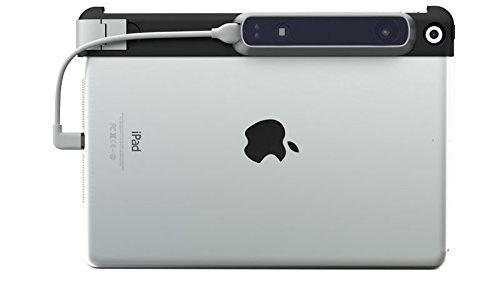
\includegraphics[width = 12cm]{Figures/ipad.jpg}
    \caption{Structural SensorImage Scource: Amazon.com}
    \label{fig:Structural_Sensor}
\end{figure}{}

Having a rich scene understanding of indoor spaces can answer various problems related to robotics, human activity recognition etc. also in some of the immersive experience and interactive technologies like  virtual reality and augmented reality applications where positional tracking and scene knowledge is crucial.

One of our interest is to achieve a good scene understanding related to depth information for indoor environment. This might open the doors of opportunities for various multimedia applications where depth information could be very crucial. One such example is \textit{IKEA Place} - an application developed by Apple in partnership with Ikea. \textit{IKEA Place} helps you to measure and place a 3D model of furniture from the Ikea catalog \cite{lehnert2017neue}. The furniture is represented as a 3D model in camera-enabled mobile device in this application \textit{IKEA Place}. One can walk around, bringing the piece of furniture in your camera-enabled mobile device and look at it from all sides and see where it can fit in your new house. This is one of the application where depth information could be used. To look at this concept of \textit{IKEA Place} in different perspective, we can recreate the entire indoor space as a 3D model and one can modify each element of their living or working spaces in a personalized fashion. This is one of the example idea where the depth information and 3D reconstruction of a indoor environment concepts can be used, this can be scaled up for various other application as well. Hence the applications of 3D reconstruction of indoor environment can have a wide range of usability. Similarly to the above mentioned application of 3D reconstruction, consumer level usability is also our main focus when applying depth estimation methods.  This is because, even though various efficient methods has been proposed based on the projection of structured light (as discussed in introduction and will be discussed in section \ref{Chapter3:RelatedWork} in detail) are available, the application at the consumer level might be challenging with respect to configuration, portability and background knowledge for usability. As we are discussing at consumer level usability, one of the areas we can look into is portable mobile device cameras. Nowadays, vast majority of cameras distributed in the market are embedded in mobile devices. These cameras have constraints on physical size, mechanical parts and processing capacity \cite{lee2007constraints}. Photographs from portable mobile devices are found to be a new approach for 3D reconstruction besides various traditional sensor based methods \cite{micheletti2015investigating, adan20113d}. In other words 3D image reconstruction from 2D images is our focus and motivation to find a solution in this area. In this context, in our project we utilized Structure Sensor manufactured by company called Occipital which is as SLS for portable mobile devices like Apple IPads as shown in figure \ref{fig:Structural_Sensor}. This comes with an additional hardware installation. Also there have been some efforts made towards low cost and efficient indoor 3D reconstruction using images collected with portable mobile devices or consumer level cameras \cite{ding2019low} but often time these accuracy or quality of these methods always have a trade off with resources like hardware (using SLS, camera quality) or computational efficiency.

In summary, as we understand the importance of depth estimation and its possibilities of remarkable applications in various areas, our motivation in this work is 3D reconstruction of a scene from a given 2D RGB image information which will lead to made consumer level application. For this we also want to answer if we can use brain style computational Artificial Neural Network (ANN) methods because we believe that by implementing a software based method might reduce the complexity at users end but with a trade off of computational power. With the growth of computational power, we believe that it is very much plausible to implement ANN models to consumer level applications in near future.

\section{Topic Description}
\label{Chapeter1:Topic_Description}
\begin{figure}[h]
    \centering
    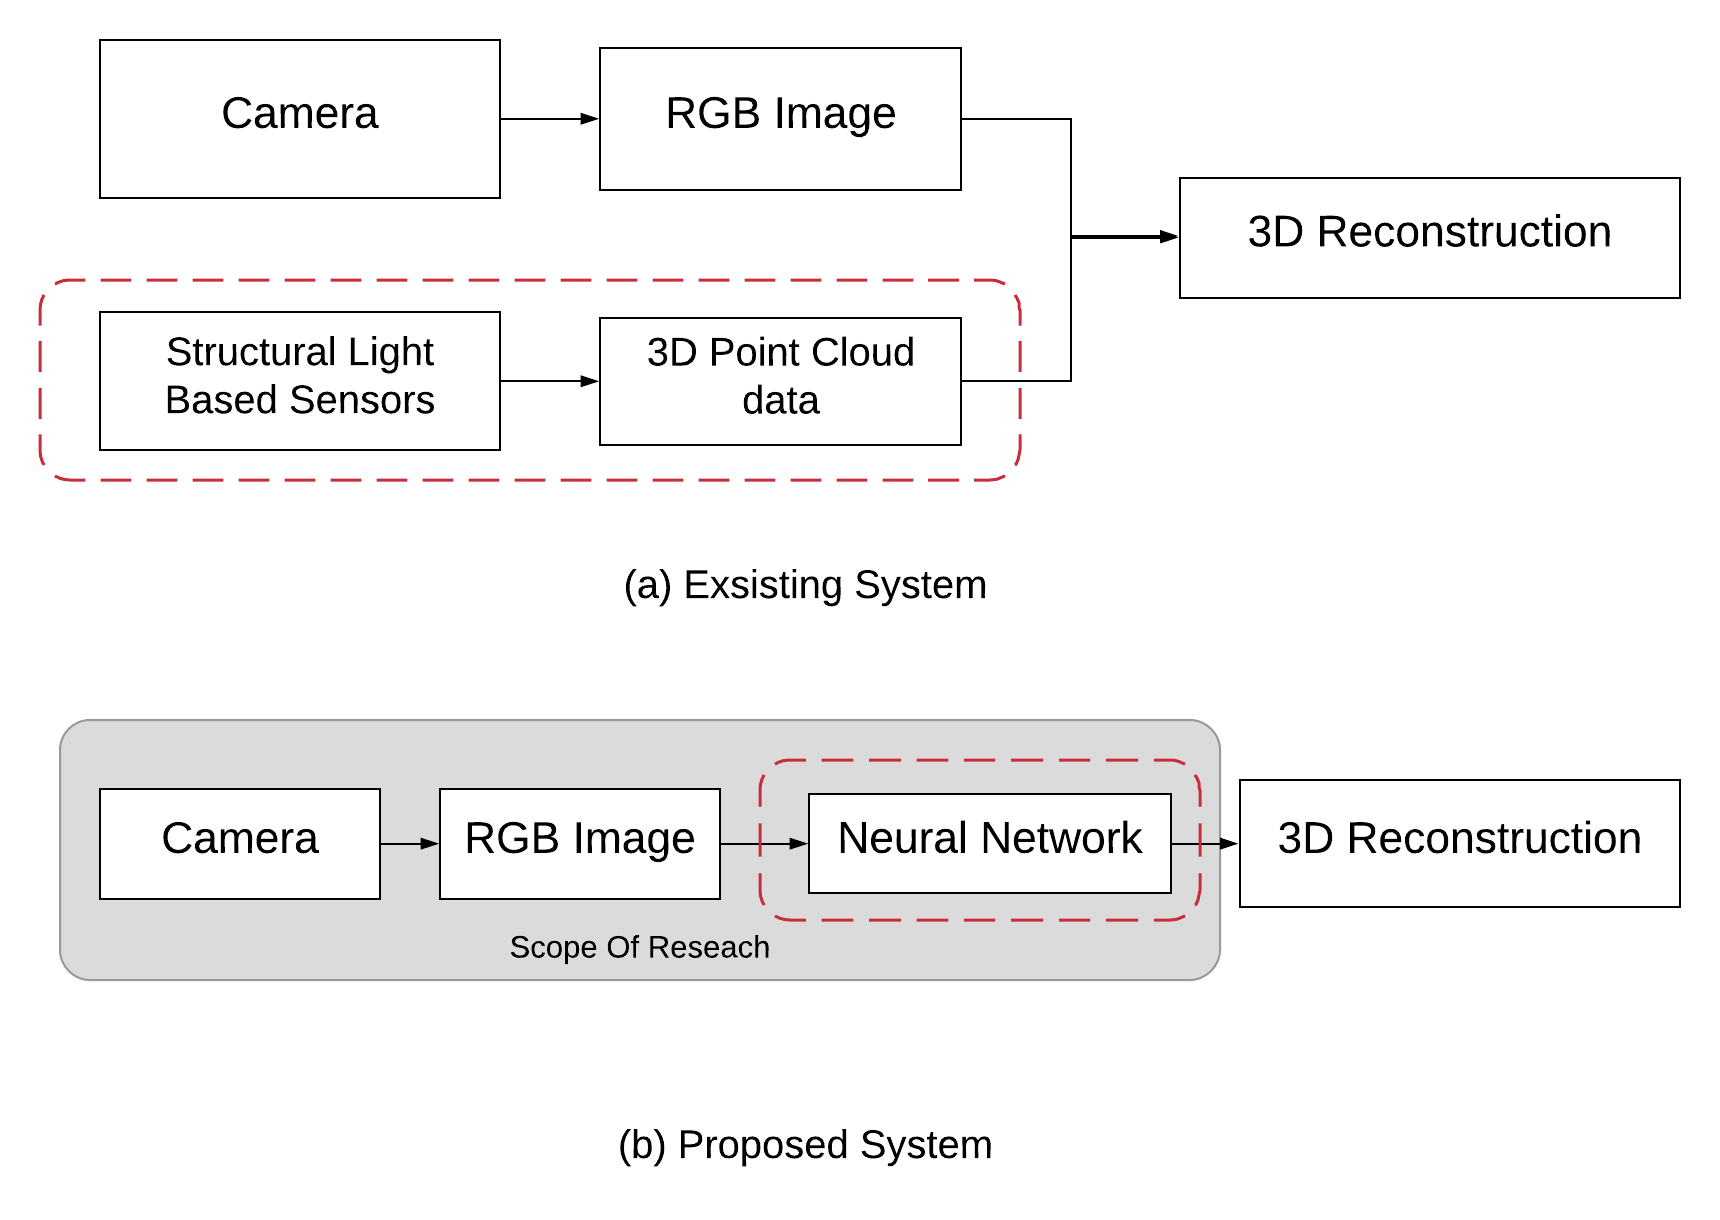
\includegraphics[width = 12cm]{Figures/idea.png}
    \caption{Topic Idea: The highlighted region in red box from existing system (a) is replaced by highlighted region in red box in proposed method (b)}
    \label{fig:Proposed_Model}
\end{figure}{}
%1-2 page(s): What are you doing?
This study proposes neural networks as an algorithm of depth estimation, more specifically using Convolutions Neural Networks(CNNs). The solution should define concise and accurate pixel for 3D reconstruction. Therefore, the goal is to achieve high accuracy in identifying the depth, especially boundaries of closer objects since the application is in indoor environment. Meanwhile, keeping the network operating speeds at a satisfying level, but the final implementation of this network will be on larger processing unit not in mobile device. This could be achieved by choosing a network architecture wisely with an attention to the details of the problem. Monocular depth estimation is based on ex-ploiting both local properties of texture, gradients, and color, as well as global geometric relations, like relative object placement, and perspective cues \cite{saxena2006learning}. Hence having a global structural understanding of image by Neural Network is very important and at the same time pixel level details for smaller object is also important in a scene. Often times the indoor environment could be more complex than outdoor because of several smaller objects in a scene. For example in office environment, there could be various physical objects on the table where as in outdoor environment having to deal with relatively larger object dimensions are more common.  

Aim of this project is to deliver a robust method and an architecture for depth image prediction replacing the sensor. As shown in figure \ref{fig:Proposed_Model} (a) Existing System for 3D reconstruction rely on hardware based implementation of a SLS which in our case is Structure Sensor integrated with Ipad as seen previously in Figure \ref{fig:Structural_Sensor}. This is done using Apple AR kit implementation which gives 2D RGB image from IPad and its depth information from the Structure Sensor and together are sent for further processing of 3D reconstruction. Thus our primary goal is to replace the existing system highlighted in red box as shown in Figure \ref{fig:Proposed_Model} (a) which consists of the structural light based sensors and the 3D point cloud data with a Neural Network as shown in the highlighted box in Figure \ref{fig:Proposed_Model}(b). We take advantage of Neural network as this has proven to give great results which we will see in details in section \ref{Chapter3:RelatedWork}.


Secondly, existing solutions to depth estimation from a single image usually rely on assumptions in which all the far field depth are mapped to a certain threshold which can result as a wall in 3D reconstruction from 2D. For example, the depth range of Kinet v2 sensor range from 0.5 meters (m) to 4.5m, which means that Kinet has a threshold that maps range above 4.5m to the maximum value of 4.5m that in turns results a wall. \cite{Silberman:ECCV12}. In practical implementation for 3D reconstruction its undesirable for us to have wall. Whereas the possibilities of the the output from SLB or Kinet sensors might give a inaccurate depth and most often times dead pixel - which is also called as holes for range above any threshold (for Kinet v2 is 4.5m) \cite{kinecttof}. Another very important reason for having holes is to get perfect reconstruction - ideally we can repaint the holes by changing the position of camera and not by any post processing methods which gives us better pixel level accuracy than in painting it, hence rather than approximation the values around holes, it is important for us to have information about these holes. In our work we are also interested to address this problem. We wanted the the network to learn these holes mimicking the SLS along with the relative depth of the scene for efficient regeneration of 3D scene. 

Thirdly, We were also interested to study about the effect of different camera and sensor properties in depth estimation mimicking the  Structure Sensor. This is because as we discussed earlier there are various types of SBL sensors avalable which has different properties. We will discuss in detail about these differences in following section \ref{Chapter4:Dataset}. Another reason for this study is because, most of the indoor scene depth estimations are based developed based on the dataset created by Kinet sensors, one such example is NYU\_v2 dataset \cite{silberman11indoor} which We will also discuss more in detail in related work section \ref{Chapter3:RelatedWork}. Thus Structure Sensor and Kinet sensor have different properties with respect to both sensors and cameras (which is used to map the relative color pixel) which brings us to a question how a Neural Network trained on different dataset influence the depth map suitable for images from IPad.  

These three problems gives us a clear direction to formulates some of the specific questions to be answered in this work which is described below. 


\section{Research questions and scientific contributions}
%1 page: Hence, this thesis tries to answer the following research question(s):

This work tries to address the following two questions:
\begin{itemize}
    \item RQ1: Can a Neural Network mimic SLS in predicting relative depth of a scene?
    \item RQ2: Can a Neural Network learn to regenerate the holes from a given depth information available from ?
    \item RQ3: Can a Neural Network learn Different Camera intrinsic and extrinsic parameters?  
\end{itemize}

In order to answer the three questions mentioned above, we propose a state-of-the-art approach using neural networks for this problem. Also generation of a new dataset is required to answer RQ2 and RQ3. This is because our goal is to achieve a model which replaces a specific SLS which is Structure Sensor and also most of the approach does not focus in retrieving the holes and existing dataset like Cornell Dataset \cite{3Dscene} , Washington Data V2 \cite{Washington}, Berkeley 3-D Object dataset (B3DO) \cite{Janoch:EECS-2012-85} etc. fail to provide with the holes except NYUv2 dataset with contains raw data information we will discuss more about the dataset in detain in section \ref{Chapter4:Dataset}. To give a justified reason for RQ3, we need to generate new dataset to have a common ground for comparison. 

Our three main contributions for this work are first, proposed a neural network model for depth map generation and compare with state of the art results. Secondly to deliver model which performs as good as Structure Sensor. Thirdly,  we created a new dataset based on Structural (SLB) Sensor.

Ultimately aim to achieve a similar working neural network model replacing Structural (SLB) sensor. This might reduce the complexity in users with a trade off of computational power. In the initial phase of this research our scope of study is to generate the 3D depth maps from neural networks after training on similar depth data. All the computation and evaluation were performed and tested with high processing unit which is described in details in Section \ref{Chapter5:HardwarSoftwareDetails}.



% Chapter Template

\chapter{Basic Principles}
\label{Chapter2:Background} 

In this chapter we  discuss the basic  principles needed for this work. The entire chapter is divided into two sections. In the first Section we go through some theory of neural network and basic building blocks needed for designing a proper neural network. Most of the concepts related to ANNs are taken from the book by Friedman et al. \cite{friedman2001elements}. The Second part will be comprising of some basics of depth estimation and camera parameters concepts. Since the area of Artificial Neural Network is very vast we will be focusing on the concepts which was specifically used for this study. 

\section{Artificial Neural Networks}

ANNs are developed algorithm similar to brain style computation which consists of different levels of neurons and capable of learning from different data. In other words we can say its a statistical learning or science of learning from given data. There are various types of learning approaches for solving problems regarding optimization . However, deep learning methodologies have proven to be favorable for many computer vision tasks related classification, detection, prediction etc.\cite{friedman2001elements} 

To understand the basics we first consider the two major types of Neural Networks which are supervised learning and unsupervised learning. In general, we denote \(X\) as input and \(Y\) as output of a given function. For supervised learning, the labels \(y_{i}\) for each input example \(x_{i}\) where    \(\{(x_{1},y_{1}),(x_{2},y_{2}),...(x_{n},y_{n})\} \in X\) for a learning algorithm satisfying function \(f:X \rightarrow Y\) and in such a way that the output \( \hat{y_{i}} = P (y_{i}|x_{i})\) where the output is depended upon the input. All labeled problems can be categorized under supervised learning. For  unsupervised learning, clustering or grouping is basically defined as the detection of similarities and joint density \(Pr(X)\) for a given input examples \({(x_{1},x_{2},...,x_{n})} \in X\) . In supervised learning there is a definite score of success which is \(P(y|y)\) \cite{friedman2001elements}. 

We can understand more about supervised learning with the help of simple binary logistic regression model which is given by
\begin{equation} \label{equation:feedforward}
    \hat{y_{i}} = x_{i}W + b 
\end{equation}

In our study we used supervised learning with convolutions network. To have a basic understanding, we discuss few nuts and blots concepts of CNN. The basic building block for a simple CNN is the filter. For the naming convention we use \textit{kernel size} for expressing the size of each filter which will be used throughout this thesis to denote filter size and not to be confused with number of filters. Idea of using filter could be easily understood when related to an example approach for finding edges in an image using a filter designed for edge detection or applying some Gaussian blur. But these filter which are represented in a matrix or in tensor form can be changed, updated or transformed based on \(W\) and \(b\) which is described in equation \ref{equation:feedforward}. Applying these filters in fashion of a sliding window, the network is converting an entire image to a space of the filter which depends on kernel size and also the step of the window slide which is also called as stride. For feature learning methods and filter space adaptation, various attribute contributes to this learning process such as forward propagation and weight \(W\) updates during back propagation which in turn modeled based on various loss function using optimization methods. An optimizer is basically a minimizing error function. In simple terms it is a error function which helps us to improve our results. Finally in order to tweak the training and optimize the learning progress we have various parameters called hyper-parameters. Some of these parameters are learning rate, in the case for gradient descent approach, decay rate which defined the descent rate after one iteration over entire training set, various regularizes and also some regularization term to prevent over fitting of the neural network model \cite{friedman2001elements}. 

%where b \in\mathbb{R}



\section{Depth Estimation}
3D spatial awareness have become more and more important with emerging technology of Augmented Reality and Virtual Reality. These 3D scanners use different approaches to estimate the depth out of a scene. Some of the major approaches being used are Stereo Imaging \cite{stereoimaging}, Structured Light System (SLS), Structure from Motion (SfM) \cite{sfm}, Time of Flight (ToF) \cite{timeofflight} and Laser Triangulation \cite{3DLasertechnique}. These approaches either use single frame or multiple frame to generate the third dimension depth. For example, SfM perceives the depth using motion cues alone where it takes multiple frames and with different point of views of the object to determine the the motion cues\cite{sfm}. This not only needs heavy computation but is time consuming as well. On the other hand, Stereo Imaging computes a Disparity map by matching features of left and right image to calculate the depth of objects with the help of only two images \cite{stereoimaging}.

\begin{table}[h]
\begin{tabular}{@{}lll@{}}
\toprule
\textbf{Technique}                    & \textbf{Advantage}           & \textbf{Disadvantage}         \\ \midrule
Structure from Motion          & High capture frequency & Time consuming                 \\
Time of Flight       & No effect of lighting & Low capture frequency     \\
Structured Light System        & High resolution   & Prone to noise                 \\ 
                            &                     &                                               
\end{tabular}
\caption{Comparison of different 3D Scanning Techniques} 
\label{table:3DScanning}
\end{table}


ToF cameras work dynamically through the scene. They scan the environment using illuminating it with incoherent light. To measure the depth, the time taken by the light to reflect back to the sensor is noted. Although ToF cameras are fast, they are often not accurate. For more accuracy we need more time and hence it only works better with static objects. \cite{tof2}.The comparison between these techniques can also be seen in Table \ref{table:3DScanning} .These techniques are now widely being used to produce 3D scanners. For example Microsoft Kinect V2.0 uses ToF technique \cite{kinecttof}, while Structure Sensor by Occipital uses SLS \cite{Kalantari}.\\

Structure Sensor (2014) is an open source integration to mobile devices which can capture depth information using Structured Light System (SLS). It consist of a laser-emitting diode, infrared radiation range projector and an infrared sensor to sense the projected radiation. The infrared sensor records the reflecting intensity of the infrared (IR) light pattern projected by the IR projector onto the target while its system on the chip (SOC) triangulates the 3D scene  \cite{Kalantari} (As seen in Figure \ref{fig:Structuresensor}). Prime Sense chip (Heindl 2014) is used as the system on the chip (SOC) in Structure Sensor. The hardware can be easily installed to the mobile device through a customized USB 2.0 connection and Structure Software Development Kit. The micro lenses in the projector have different focal lengths which produces a non-uniform pattern of dots which varies at different distances \cite{Kalantari}. \\


\begin{figure}[h]
\centering
    
\includegraphics[scale=0.29]{Figures/illustration-of-structure-sensor.png}
    \caption{Illustration of Structure Sensor}
    \label{fig:Structuresensor}
\end{figure}

The biggest advantage of Structure Sensor over any other available depth camera is the size of the hardware. As it is only 120mm long and 28mm wide, One can easily fit Structure Sensor in their pockets. Another advantage of it is that for small rooms and office environments it gives us reasonably good results. Looking at our scope of research, we would also like to fully utilize the integration to a mobile device as well since our end goal is to make the network compatible to mobile devices. These features altogether makes Structure Sensor a perfect choice for our project.\\ 
% Chapter Template

\chapter{Related Work} % Main chapter title

\label{Chapter3:RelatedWork} % Change X to a consecutive number; for referencing this chapter elsewhere, use \ref{ChapterX}

%----------------------------------------------------------------------------------------
%	SECTION 1 4+ pages
%----------------------------------------------------------------------------------------
In this chapter we discuss about various recent state of the art approaches and methods for estimating Monocular depths using deep neural networks (DNNs). We will be discussing about different earlier approaches on this subject in section \ref{Chapter3:RelatedWork_EarlyApproach} briefly and look into more specific and elaborated details in recent approaches using Neural Networks based on different important factors in section \ref{Chapter3:RelatedWork_NNModel}. We have also discussed about various datasets which are available. 

\section{Early Approaches}
\label{Chapter3:RelatedWork_EarlyApproach}
Understating of structural orientation of a object in an image, recovering range and object depicted in an given image is one of the basic problems scene understating. Many traditional approaches mainly focus on low-level image cues and geometric structures - most often handcrafted method \cite{torralba2002depth, pentland1987new,lai1992generalized,saxena2006learning}.
 
One of the very early approaches on image understanding with respect to reconstruction of depth image can be traced back in 1982 Barnard et. al. \cite{barnard1982computational} where they discussed various state-of-the-art computational methods for recovery of depth images at that period of time, which mainly focus on two aspects which are camera geometry and disparity mapping. Later in 1987 Stephen T. Barnard proposed a stochastic approach which provides a dense array of disparities, eliminating the need for interpolation \cite{barnard1987stochastic}. After that D. Scharstein and R. Szeliski \cite{scharstein2002taxonomy} came up with a taxonomy for dense two-frame stereo correspondence algorithms.\\

\subsection{Probabilistic Models}
\label{Chapter3:RelatedWork_ProbabilisticModel}
Probabilistic Models were the initial steps towards DNNs. Sexana et al. \cite{saxena2006learning} in 2006 were one of the first to propose an probabilistic model to predict depth image from single image. This approach was based on Markov Random Field (MRF) using Gaussian and Laplasian distribution model. Features were considered on small patch level of a given image \footnote{images were sub divided into small patches} in two distinctive levels. First, to estimate the absolute depth and second to estimate relative depth. This relative depth were calculated based on magnitude of the difference in depth between two patches for which three different local cues such as texture variations, texture gradients and haze were considered. Distance 3D scanner were used for data collection for this purpose. Their work was extended to 3D scene reconstruction with improved MRF model, Make3D \cite{saxena2008make3d} system for 3D model generation. One of the challenges of this system is that the images relies on horizontal allied calibration. 

This work lead to various new probabilistic models which in recent years can be classified into Deep Neural Networks (DNNs). Recent years many solutions has be tried for monocular depth estimation problem such as supervised, semi-supervised and unsupervised learning.   

One of the inspiring modern approach by Eigen et al. 2014 \cite{eigen2014depth} where two network component stack were used namely global coarse-scale network followed by local fine-scale network. Global coarse-scale network predict overall depth structure which is intern then refined by a local fine-scale network. This opened doors for fusing feature maps from different level for better predictions.
Also many Convolution Neural Networks (CNNs) based models where used to understand the relationship between RGB images and its corresponding depth maps \cite{liu2015deep,laina2016deeper,Eigen_2015_ICCV,eigen2014depth, Alhashim2018}. By this time encoder-decoder style of architecture where famous\cite{Alhashim2018, hu2019revisiting} which we will discuss in detail in section \ref{Chapter3:RelatedWork_NNModel}. 

Meanwhile some other works focused of various other details like,  Ladicky et al. \cite{ladicky2014pulling} highlights the limitation of the various data driven approaches for monocular depth estimation by exploring the structural perspective  geometry. Zammir et al. \cite{zamir2018taskonomy} studied on the modeling structure space of visual task and investigating on transfer learning dependencies, one of the finding where, the demand of labeled dataset could be reduced by introducing transfer learning approaches since there is always model and structural dependencies. Ha et al. \cite{ha2016high} also proposed a high quality depth map from non calibrated short video clip. Shu et al. \cite{Shi2015BreakAR} proposed that small-scale de focus blur can enhance the depth prediction and Fouhey et al. \cite{Fouhey_2013_ICCV} also tried to learn structural component.




\section{Recent Neural network Approach}
\label{Chapter3:RelatedWork_NNModel}
 Remarkable advances has been made in deep learning Laina et al. \cite{laina2016deeper} proposed a new architecture build on ResNet-50 by replacing the last layer with up sampling layers for reconstructions. They also proposed new loss function \textit{Huber Loss} an end to end approach, model can learn geometrical relationship. In the same way some approaches replaced ResNet backbone by different pretrained models as encoder\cite{Alhashim2018, hu2019revisiting}. More recent work focused on combining information from multiple scale, encoder and decoder style. This is to get the different level learned features \cite{Xu_2018_CVPR, Eigen_2015_ICCV} then concatenated at the decoder part of up sampling stage of architecture. One of main reason for such approach is to get higher spatial resolution by eliminating distorted and blurry edge since the probabilistic distribution always results into smooths object boundaries\cite{hu2019revisiting}. Also having features learned from top layers contains higher level information like which can give a global understanding of structural aspect of a image or scene. Meanwhile there where also some unsupervised learning methods applied for the same task \cite{godard2017unsupervised, qi2018geonet}.

We have analyzed the resent work in detail and will be describing more about different approaches categorizing into three groups model architecture, input representation and dataset used. These are the most commonly known to be the most important factors which defines the performance of a Network.

\subsection{Model Architecture}
\label{Chapter3:ModelArch}
In recent years since many encoder-decoder and multi scale style proven to give better results \cite{Alhashim2018, hu2019revisiting}. In this work we have used the similar architecture. In these encoder-decoder architecture the encoder always comprises of a backbone of a larger pretrained model. The most common encoder backbone which could be found are Residual Network (ResNet), Densely Connected Convolutional Network (DenseNet), Squeeze and Excitation Network (SENet) or Visual Geometry Group Network (VGGNet)\cite{hu2019revisiting}. Deep neural network with large number of layer are difficult to train due to vanishing and exploding gradient. ResNet helps to skip intermediate identity connections by 
\begin{equation} \label{eqResNet}
    {a^{i+n}=g(z^{i+n} + a^i)}
\end{equation}


where \(g\) is the non-linear activation function (eg. ReLu) and \(z\) is the output of linear activation (or output of a particular layer) of $i^{\text{th}}$ layer and \(a\) denotes the output of a layer. In contrast, DenseNet is an extension of ResNet where instead of skipping the and merging with the $i+n^{\text{th}}$ layer as an addition, DenseNet performs concatenation of all the $n$ skipped feature maps
\begin{equation} \label{eqDenseNet}
    {a^{i+n}=g(z^{i+n} + a^{C})}
\end{equation}


where \({C =C_i([i,i_2,...,i_{n-1}])}\) denotes the concatenation of \(i^{th}\) layer till \(i_{n-1}^{th}\) using the summation \cite{huang2017densely} there by helping feature propagation, feature reuse and  reduce the parameters. Where as SENet is a transforms a set of block to another. It comprises of squeeze operator and excitation operator. Squeeze operator aggregates the feature map and excitation operator  aggregates the learned activations Net \cite{iandola2016squeezenet}. 


We compare 6 different neural network architecture as tabulated in table \ref{table:RelatedWork_STA_Architecture}. These models are selected based on the most recent approaches from years  2018 - 2019 and sorted based on the Root Mean Squared Error (RMSE). All the RMSE score are based on test set of NYU v2 depth map dataset \cite{silberman11indoor}.

\textbf{M1}, \textbf{M3} and partially \textbf{M4}, were build upon ResNet backbone for depth prediction. Even though all the three methods are different, \textbf{M3} and \textbf{M4} methods have one thing in common which is that both architecture were designed for multi-task specific model after encoder-decoder part. \textbf{M3} Pattern Affinitive Propagation (PAP-Depth) method idea was developed based on the affinity behaviour between two similar task \footnote{for example finding Surface normal and depth are related task, These two factors remains the  most important component for image segmentation}. This can be described by Affinity Block or sub network, which comes after the up-sampling (decoder part). The last layers are fed into three different task-specific networks for prediction of Depth, surface normal and segmentation. They also integrate multi-scale features derived from different layers of encoder each with a task-specific network. Each task-specific network has two residual blocks, and produces the initial prediction after a convolution layer. Then conduct cross-task propagation to learn the task-level affinitive patterns. Each task-specific network initially learns an affinity matrix by the affinity learning layer to capture the pair-wise similarities for each task.

\textbf{M3}, SharpNet basically was built for addressing pixel-perfect near occluding contours  problem. The approach of SharpNet is very similar to \textbf{M4}. Instead of segmentation sub-net, SharpNet has occluding contours as one among the three 3 multi-task network model after the decoder part. The features from encoder is integrated to this sub-network. 

\textbf{M1}, Geometric Network (GeoNet) is a two layer architechure - built upon two two big CNN model (ResNet and VGG) in two different blocks. In first block the two models (ResNet and VGG) are trained separately. VGG is used for depth images and ResNet for surface normal prediction of a image. The output is given to second block which consist of two sub network namely \textit{Depth-to-Normal} and \textit{Normal-to-Depth}. As the names suggested, the depth output from VGG is fed into \textit{Depth-to-Normal} to enhance the quality of surface normal while on the contrarily the \textit{Normal-to-Depth} sub network receives surface normal from VGG and improves the depth map.


\textbf{M2} and \textbf{M6} are built upon DenseNet backbone. In \textbf{M6} one of the distinctive idea is, the decoder part has multiple resolution block. If \(\textbf{\textit{$B_n$}}\) is denoted as one block of decoder to obtain output resolution of \(\textbf{\textit{$D_n$}}\) , then  \(\textbf{\textit{$D$}}\) depends on number of  \(\textbf{\textit{B}}\). In this approach they have 5 different resolution \(\textbf{\textit{$D_n$}}\)  such that \(n = 5\) for extraction of multi resolution depth from different positions to get relative depths. Final depth image is obtained from relative pair-vise comparison with the relative depth images from different \(\textbf{\textit{$B_n$}}\).

\textbf{M2} DenseDepth is a much simpler model than all the above approaches yet proven to have best results than others in terms of RMSE on NYU dataset. There are two distinctive  ideas. First, they use multi-scale encoder featured concatenated with decoder part to get a better structural higher level features, also the decoder is made of \(2 x \) bilinear up sampling method. Second, they use transfer learning approach.  

\begin{table}[t]
\centering
\begin{tabular}{p{0.05\linewidth}p{0.2\linewidth}p{0.1\linewidth}p{0.3\linewidth}p{0.2\linewidth}}
%{|c|c|c|c|c|}


\hline
\textbf{\# } & \textbf{Method} & \textbf{RMSE} & \textbf{Backend}& \textbf{Year/Reference} \\ \hline\hline
M1              & GeoNet          & 0.445             & ResNet and VGG  & 2018 \cite{qi2018geonet}          \\ \hline
M2              & DenseDepth      & 0.465             & DenseNet        & 2018 \cite{Alhashim2018}         \\ \hline
M3              & SharpNet        & 0.496             & ResNet       & 2019 \cite{ramamonjisoa2019sharpnet}\\ \hline
M4              & PAP-Depth       & 0.497             & ResNet          & 2019 \cite{Zhang_2019_CVPR}         \\ \hline
M5              & SENet-154       & 0.530             & SENet           & 2018 \cite{hu2019revisiting}          \\ \hline
M6              & RelativeDepth   & 0.538             & DenseNet        & 2019 \cite{lee2019monocular}          \\ \hline
\end{tabular}

\caption{Investigated neural network architecture on Monocular Depth Estimation on NYU\_v2 Dataset}
\label{table:RelatedWork_STA_Architecture}

\end{table}


There are some advantages of using DenseNet over ResNets. Firstly, there is a strong gradient flow because increase in the depth of a CNN might result in vanishing gradient problem . Second, we get more diversified feature, which means there can be good generalized information from the previous layers which tends to have richer patterns whereas in skip style ResNet such information are lost. 

In summary, despite of having simpler model by Alhashim et. al \cite{Alhashim2018}  the results which are reported seems to be more convincing even when being compared with various other complex and big models. Among these literature, it is found out that the most common encoder backend for encoder-decoder style nerwork are  ResNet and DenseNet. Both of them have proven to have to least error value among our comparative study. Inspired by the simplicity and the results of  Alhashim et. al. work on DenseDepth we use DenseNet model as backbone encoder in our work for estimating depth maps. We would like to highlight three distinctive reason for selecting this approach. First as we see DenseNet have proven to have some advantages over for deeper network by having temporal feature information of the skipped layers. Second the model uses transfer learning and trained 120,000 images from NYU v2 datased which weights have be shared to public Which reduces the computation needed for re-training the decoder architecture again. Third, many recent models have various multi-sub task network and for such approches computational time also adds an important factor, in our case we are more focused in Structure Sensor in a RGB-depth map pair training for depth estimation as described in section \ref{Chapeter1:Topic_Description}.


\subsection{Input Representation}
One of the important aspect of feature based learning is input representation of a feature to its respective model \cite{friedman2001elements}. The most common approach of input representation is in its simple form of RGB and depth pair from various SLS sensors \cite{eigen2014depth, xu2017multi}. Some approaches also exploits the structural orientation by computing surface normal \cite{li2015depth, qi2018geonet}. One of the approach Zhang et. al. \cite{Zhang_2019_CVPR} was to utilize three features:  depth, surface normal and segmentation which then fused together by concatenation and given as input at encoder whereas at the decoder part a multi-sub task specific network was designed. The advantage of such multi feature is it can have a good cross task learning - which means different features can be represented for the same temporal content. One more example of  cross task learning is \cite{qi2018geonet} when two models are used for two different input feature: depth image and surface normal. Another type of input which was used in some approaches is sparsity  \cite{chen2018estimating, mal2018sparse}. Chen et. al. \cite{chen2018estimating} computed the sparsity matrix and given as an addition input along with depth maps. In our work we used the most common approach RGB - depth map pair as input feature.  

\subsection{Existing Datasets}

One of the most important component in feature based learning methods are highly dependent on data itself \cite{friedman2001elements}, which mean the result of such probabilistic output models can be highly influenced by the dataset itself. For example, We can either fit a model by training with the small amount of dataset to perform few particular designated task in a designed environment or we can train a model on a large and diverse database to perform more generalized tasks.

There are several datasets readily available for different purposes. One of the major classification of dataset for depth maps can be classified as either by the environment scene - indoor and outdoor environment or based on application, for example KITTI for Autonomous driving \cite{Geiger2013IJRR} scenario and Berkeley 3-D Object Dataset (B3DO) \cite{Janoch:EECS-2012-85} is soulely focused for Object Recognition.

Saxena et al. \cite{saxena2006learning} proposed a dataset of 959 Images of RGB and laser range data. All the depth data was collected using a custom-built 3D laser scanner. The images are of dimensions 2272 $\times$ 1704, while the depth maps are 55 $\times$ 305. Later, Silberman et al. \cite{Silberman:ECCV12} proposed a high quality Kinect dataset (NYU Depth-V2) in 2012 which is now being used widely across the in 2012. NYU Depth-V2 \cite{Silberman:ECCV12} consist of 1449 densely labeled pairs of aligned RGB and Depth images. By labeled pair we refer to segmentation of all the surfaces with respected surface normal. Furthermore, it consists 407024 unlabeled frames. Former NYU dataset(NYU Depth V1) \cite{silberman11indoor} consisted of only 67 scenes while NYU Depth-V2 consist of 464 different indoor scenes. Both the images and Depth maps are 640 $\times$ 480 in resolution. The dataset is appreciated for the segmentation of a room.

Geiger et al. \cite{Geiger2013IJRR} in 2013, proposed an outdoor dataset consisting of stereo depth images as the KITTI Dataset. KITTI Dataset is used for Autonomous Driving and Robotics purpose. It includes high resolution color and grayscale stereo camera images, laser scans, high-precision Global Positioning System(GPS) measurements and Simultaneous Localization and Mapping (SLAM) data. The main intend was to push forward the development of computer vision and robotic algorithms targeted to autonomous driving.

In 2016, Mayer et al. \cite{MIFDB16} produced three synthetic datasets called Scene Flow Dataset providing over 35000 stereo frames with dense ground truth for optical flow, disparity and disparity change, as well as other data such as object segmentation. The resolution of these images is 960 $\times$ 540. MPI Sintel \cite{Butler:ECCV:2012} is also a synthetic depth dataset which is available online. All these dataset were created using the open source 3D creation suite Blender.

Another traditional approach to collect dataset is using crowd-sourcing. Chen et al. \cite{DBLP:journals/corr/ChenFYD16} introduced "Depth in the Wild" dataset in which they took images from Flickr \footnote{ \url{www.flickr.com}}  and presented the crowd-sourced workers with these images with two highlighted points asking which of the point was closer. The dataset consists of 495,000 diverse images, each annotated with randomly sampled points and their relative depth. 

\begin{table}[]
\begin{tabular}{lllllll}
\hline
{\textbf{Dataset}}         & \textbf{RGB size}           & \textbf{Depth size} & \textbf {\# of images} & \textbf{References}                                  \\ \hline
Make3D  $\dagger$                     & 2272 $\times$ 1704                & 55 $\times$ 305           & 959                       & \cite{saxena2008make3d}               \\ \hline
NYU V2 $\bullet$                      & 640 $\times$ 480                  & 512 $\times$ 424          & 407,024                   & \cite{Silberman:ECCV12}             \\ \hline
KITTI  $\dagger$ & 1392 $\times$ 512  & -                         & 15,000                    & \cite{Geiger2013IJRR}               \\ \hline
B3DO  $\bullet$                      & 640 $\times$ 480                  & 512 $\times$ 424          & 849                       & \cite{Janoch:EECS-2012-85}          \\ \hline
Cornell Dataset 	$\bullet$           & 640 $\times$ 480                  & 640 $\times$ 480          & 550                       & \cite{3Dscene}                      \\ \hline
Washington V2  $\bullet$  & 640 $\times$ 480                  & 640 $\times$ 480          & 300                       & \cite{Washington}                   \\ \hline
Scene Flow  $\dagger$                      & 960 $\times$ 540                  & 960 $\times$ 540          & 39000                     & \cite{MIFDB16}                      \\ \hline
Depth in the Wild                            & -                                 & -                         & 495,000                   & \cite{DBLP:journals/corr/ChenFYD16} \\ \hline
\end{tabular}
\caption{Comparision of various datasets where $\dagger$ means outdoor, $\bullet$ is indoor and - refers to N/A}
\label{table:DatasetComparision}
\end{table}

There are many Other datasets are available like Cornell Dataset \cite{3Dscene} , Washington Data V2 \cite{Washington} and  Berkeley 3-D Object dataset (B3DO) \cite{Janoch:EECS-2012-85} also follows the same approach of labelling the environment either for object recognition or robotics purpose. All of them were also captured using Kinect camera approach producing RGB-D images. We can see the comparison of all the datasets in table \ref{table:DatasetComparision}.

As we can see, all of the Datasets mentioned above are suitable for different application scenarios. For example, NYU V2 \cite{Silberman:ECCV12} is best for Segmentation purpose, B3DO \cite{Janoch:EECS-2012-85} is suitable for Object Recognition and KITTI Dataset \cite{Geiger2013IJRR} for Autonomous Driving purpose. Keeping in mind the scope of the research is to estimate depth of monocular indoor scenarios and office environments, NYU V2 is the most relevant as it has high quality depth maps for indoor environment which can be exploited for training of the network. As discussed in Section \ref{Chapter3:ModelArch}, we produce a small dataset using a Structure Sensor to make the model more focused towards mobile devices which is discussed in next chapter.



%\section{Additional Details}
%\url{https://paperswithcode.com/sota/monocular-depth-estimation-on-nyu-depth-v2?p=high-quality-monocular-depth-estimation-via}%
%upsampling cound be in many parts

%\begin{itemize}
 %  \item Nearest Neighbor
  % \item Bilinear Interpolation,  A single pixel value is calculated as the weighted avg.
   %\item Transposed Convolution, we have weights that we learn through back propagation.
%   \item Recent works
%\end{itemize}


%Supervised 
%CNN - slam - \cite{Tateno_2017_CVPR}
%CRNN
%GeoNet

%\\
%unsupervised \\
%un supersed CNN - geometry  - \cite{garg2016unsupervised}
% Unsupervised Learning of Depth and Ego-Motion From Video- \cite{Xu_2018_CVPR}
%Left and right

%\\
%Transfer learning\\
%CNN -

%\\
%{https://github.com/GabrielMajeri/nyuv2-python-toolbox}\\
%{https://github.com/ayanc/mdepth}\\
%Some \cite{bhoi2019monocular} \cite{laina2016deeper, bhoi2019monocular}\\
%We use this curretn state of the art 

%
% Chapter Template

\chapter{Structure Depth Dataset}

\label{Chapter4:Dataset} 

%----------------------------------------------------------------------------------------
%----------------------------------------------------------------------------------------
%\url{https://fenix.tecnico.ulisboa.pt/downloadFile/1689244997256744/Thesis.pdf}

In this Chapter, We present our dataset created using Structure Sensor and we call it as \textbf{Structure Depth} dataset. The entire chapter is divided in to three sections. In the first section we discuss the technical details of the Structure Sensor and followed by the methods involved in creating this dataset. The last part of this chapter is about the various pre processing methods we used to performed for specific experimental setups.


\section{Structure Depth Dataset Overview} 

Our aim in this work is to deliver a robust system for depth prediction as seen in the Figure \ref{fig:Proposed_Model} for a portable hand held mobile device. In our case it is an Ipad integrated with Structure sensor. In order minimize the difference between the predicted depth maps and depth map generated from Structure sensor we need to train with the similar dataset. We have also validated this in our experiments which will be discussed below in Section \ref{Chapter6:Results}. As discussed in the section \ref{Chapeter1:Topic_Description}, this will also help us to study the effect of different camera and sensor properties on diffrent environment.\\

As we have seen earlier in Chapter \ref{Chapter3:RelatedWork}, there are multiple datasets available but almost none fit our context. As we are already exploiting the depth features from NYU V2 for general prediction, we would like to produce a dataset which is solely application based. Here our application is mobile device, particularly IOS, we generate the dataset using an Ipad. This will not only make the intrinsic parameters to be learned by the network but also particularize for IOS based devices. As we use Ipad as integration, all the RGB Images are received from the Ipad's camera. The features we want the neural network to learn and predict should have the same camera intrinsic parameters in order to decrease the amount of pre processing of the dataset. Hence, We first calibrate Ipad with Structure Sensor before collecting the Dataset. Another major advantage of using Structure Sensor with an Ipad over Kinect is the resolution of RGB and Depth Images. While Kinect V2 has $512\times424$ Infrared camera resolution, Structure Sensor can go upto $640\times480$. \\

Our Dataset consist of 18 scenes and a total of 2675 images captured using an Apple iPad Pro version 12.9 (2015) model and a Structure Sensor by Occipital. The dataset majorly includes images from office and classrooms environments. It consist of RGB Images of $640\times480$ as 3 channel $\times$ 8 bit int and Raw Depth Images of 640 $\times$ 480 as 1 channel. Both of the images are saved using lossless compression. Later, we also perform some processing to synchronize RGB and depth images and to fill the holes of depth image which will be discussed later in this chapter. We also provide the camera extrinsic parameters as a numpy matrix of $4\times4$ which is useful for reconstruction of a scenario.\\


\subsection{Technical Specification of Structure Sensor}
The Structure Sensor \footnote{\url{https://structure.io/}} is a 3D scanner introduced by Occipital in 2014. As the name suggests, it uses Structured-Light-System(SLS) 3D scanning\cite{Kalantari}. It can be easily attached to an Ipad and with Structure SDK it enables us to generate good quality RGB image stream from Ipad and its realtive depth stream from Structure Sensor at the simultaneously. As it only weighs 95 grams and can be used as an extension to mobile device, it makes the sensor very portable. With possibility of recording 60 frames per second at a resolution of $640\times480$\cite{Kalantari}. When compared to Kinect V2, it has more depth image resolution. The comparison can be seen in table \ref{table:KinectVsStructureSensor}. The minimum range it can capture is 40 cm while it can capture till 4 m with fine precision. After 4 m the precision is not satisfactory enough to use it for the dataset. Occipital claims it has low frame-to-frame noise and provides 100\% fill rate on most of the materials. On the other hand Ipad Pro 12.9 provides us with an RGB video stream of $1920\times1080$ at 30 frames per second and $1080\times720$ at 60 frames per second. Ipad Pro also provides us with Camera extrinsic parameters which are useful for the reconstruction of the scenario.\\

\begin{table}[h]
\begin{tabular}{@{}lll@{}}
\toprule
\textbf{Features}                    & \textbf{Kinect V2}           & \textbf{Structure Sensor}         \\ \midrule
Depth Sensor Type           & ToF & SLS                 \\
RGB Camera Resolution       & $1920\times1080$, 30 fps & $1920\times1080$, 60 fps     \\
IR Camera Resolution        & $512\times424$, 30 fps   & $640\times480$, 60 fps                 \\ 
Field of View of IR Camera  & $70^\circ\times60^\circ$           & $58^\circ\times45^\circ$                         \\
Recommended Operative Range & 0.4 m - 3.5 m       & 0.4 m - 3.5 m                                  \\
           &                     & 
\end{tabular}
\caption{Comparison of Kinect V2 and Structure Sensor}
\label{table:KinectVsStructureSensor}
\end{table}

While these sensors are great devices they have some limitations. The distance they can measure is limited and they suffer from reflection problems on transparent, shiny or very matte and absorbing objects. Another limitation is holes generated by parallax effect happening due to difference in position of the camera of Ipad and Structure Sensor\cite{Kalantari}. In simpler terms, it works like human eyes. If we close one eye and then other, we notice a disparity. When there is an object we try to focus on, we see it through different angles. If the object is close enough, then sometimes one eye can see what is behind and other can not. This can be seen in figure \ref{fig:holes}. As a result, it produces a shadow of holes which can be seen in figure \ref{fig:holes2}.

\begin{figure}[h]
    \centering
    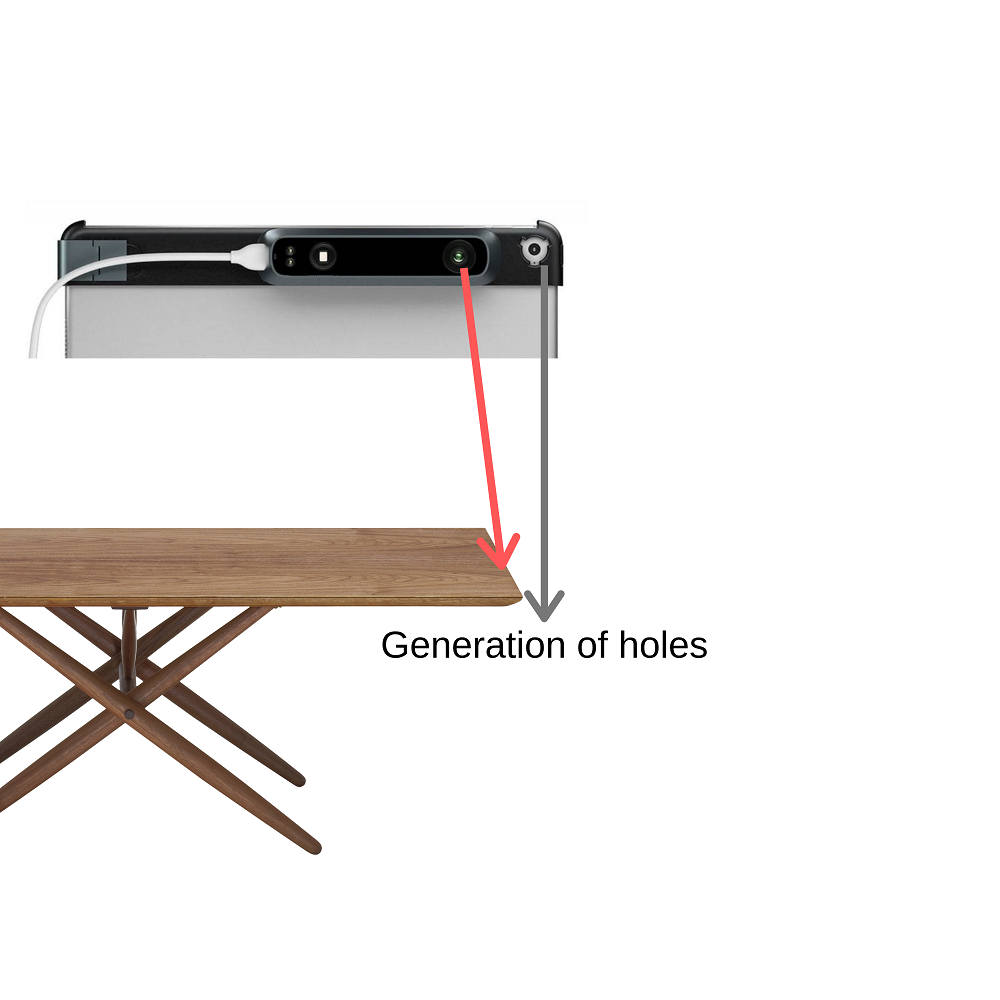
\includegraphics[scale=0.4]{Figures/holes.png}
    \caption{Generation of holes due to parallax}
    \label{fig:holes}
\end{figure}

\begin{figure}[h]
    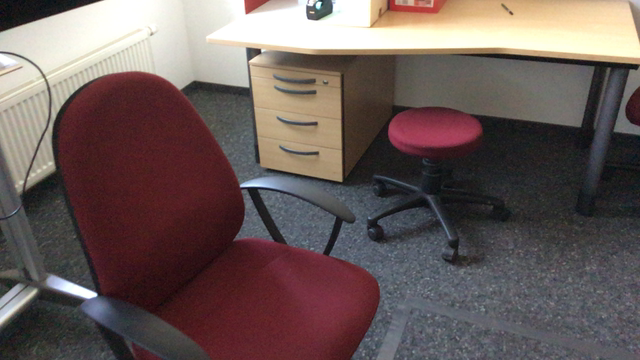
\includegraphics[scale=0.29]{Figures/RGB.png} 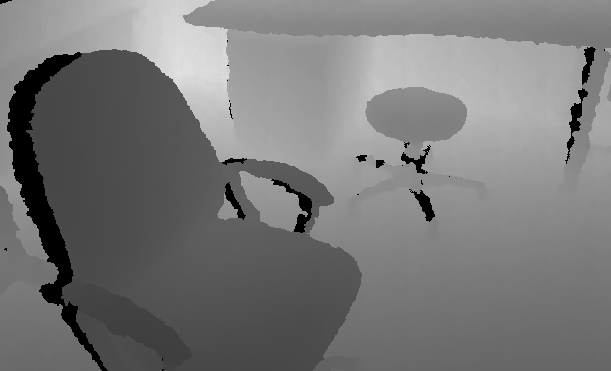
\includegraphics[scale=0.37]{Figures/Depth.png}
    \caption{Holes produced in depth image}
    \label{fig:holes2}
\end{figure}


\subsection{Dataset Collection}

A significant role in Machine Learning is played by Dataset and the collection of it makes most influence on the features that network learns. As the distance is limited in Structure Sensor and due to our scope of research we used indoor offices and classrooms to reduce the possibilities. While capturing the dataset, one should keep in mind that the network should learn only the novel features not the artifacts. One good instance of this would be recording the depth of a screen. Since, a screen has reflective black surface, it loses depth information resulting holes in depth image. \note{add img for screen} If we feed these images to the network, it might learn the features such as, screen is always at, let say x distance. Where x is pixel value we assign to such holes. This is not a good feature to be learned by the network instead it is an artifact. So before feeding it to the network we do some pre processing on the dataset which we will discuss next.\\

The generation of holes are usually due to the reflective surface of an object or the distance and position of the object\cite{geomar41830}. As a reflective/glossy surface generates holes, it should not be synthesized because this leads to distortion of depth information.

For the shadows happening due to parallax effect, we use inpainting \cite{zamir2018taskonomy} in order to minimize out the errors. Since, the accuracy decreases as the depth increases \cite{deptherror}, we remove all the pixels which are away more than 4 metres. This can be resolved using further predictions and post processing. All the information is registered in metres and  all of these processes were included while processing the raw depth information.\\

\subsection{Processing the Dataset}

After we have the distance in metres, we process the data before directly training the network on these images. Since these images still contain holes and precision less pixels, we pre process the images. Usually, very far pixels have less precision and results in holes as well\cite{deptherror}. It is a good idea to conserve those holes in order to reconstruct the environment by later predicting the future frames. Firstly, after we have the Depth images in metres, we flag \nadacn{We save all the holes by its pixel position or index} all the pixels more than 4000 cm to use them in the image later again as discussed later in this section.

As discussed earlier, the Depth images contains holes from shiny/glossy objects\cite{shiny}. In office environments, these holes are mostly generated by Computer Displays. Since we do not want our network to learn that all the screens are close(0 pixel), we interpolate these holes. We do this by inpainting the whole image. This fixes the issues of shadows made due to parallax as well. \\

In our first model, we made all the pixels more than 4 metres as 4 m like a wall but that was not a great idea. Since, our model learns what we feed it, the model now had no proper depth perception after 4 m \nadacn{this statements means after processing the depth precision  will increase more than 4 meater which is wrong} \shivam{its better to read the next line before making the comment}.\nadacn{still the statement does not convey everything.. you use "now (present tense)had (past tense) ?? I cannot corerent because I dont know what you want to say... You say, since there sensors depth sensing limitation is limited to a definite range in this case xxm the possibilities of  depth values beyond a threshold may not be with good precision, So as an approach we map all the pixel depth to a certain xx threshold... " } So, We decide to keep all the pixels more than 4 m as holes because we can reconstruct them using a video or multiple frames later if needed. Now, We have the whole image without any holes, but we want holes in our image. So, the next step is to re generate holes for the pixels more than 4000 cm. All the pixels we flagged are now changed to zero in order to create holes. \\

Our Image is now ready to be fed to the network but there is still one problem. The size of the Color Image and Depth Image does not match since they have different aspect ratios due to different camera sources. So, In the end we crop the depth image centre focused in order to make them compatible with each other.\\

\newpage 

\chapter{Methodology}

\label{Chapter5:Methodology} 
%----------------------------------------------------------------------------------------
%	SECTION 1
%----------------------------------------------------------------------------------------

In this Chapter we will discuss the entire work flow and the methods used in this study. Starting from the different model architecture and system setup describing various experimental configuration. We used two two main architecture and with some configurations to answer our research questions.


\section{System Overview}
We approached this problem of depth map estimation from monocular images to give end to end solution as much as possible using two CNN. As we discussed in the section \ref{Chapeter1:Topic_Description} our main focus was (a) to deliver a robust method and (b) regeneration of dead pixels or holes for better reconstruction of images. For this we consider two CNN models, first, we propose a model and this approach we call it as \textbf{A1} and the second model approach is a state of the art model and we call it as \textbf{A2}.  In this section we briefly describe both our models and input representation used for the experiments. And further more in order to improve our results we also propose different configuration methods. These configuration methods and motivations are described in details in the following section \ref{Chapter5:Experimental_Setup}. 


\subsection{Input Representation}
For our study we use two datasets NYU\_v2 Depth \cite{silberman11indoor} whose depth information was obtained from kinect sensor and the other dataset was created as a part of this study from Structure Sensor which is described in chapter \ref{Chapter4:Dataset}. The input dimension of target RGB images for both the approaches \textbf{A1} and \textbf{A2} are (480$\times$640$\times$3). Whereas input dimensions of ground truth depth image for \textbf{A1} is same as the target image  which is (480$\times$640$\times$1) while for \textbf{A2} is  (240$\times$320$\times$1) which is half of its target input resolution. The output depth map dimension of each approach is similar to it input.

We apply two pre-processing methods on Structure Sensor. One to train on holes and other with nearest interpolation method. Different input representation where used for different configuration which are described in details in the following section \ref{Chapter5:Experimental_Setup}.

\subsection{Approach 1 (A1) - U-Net Style Network}
\label{Chapter5:A1}
\begin{figure}[h]
    \centering
    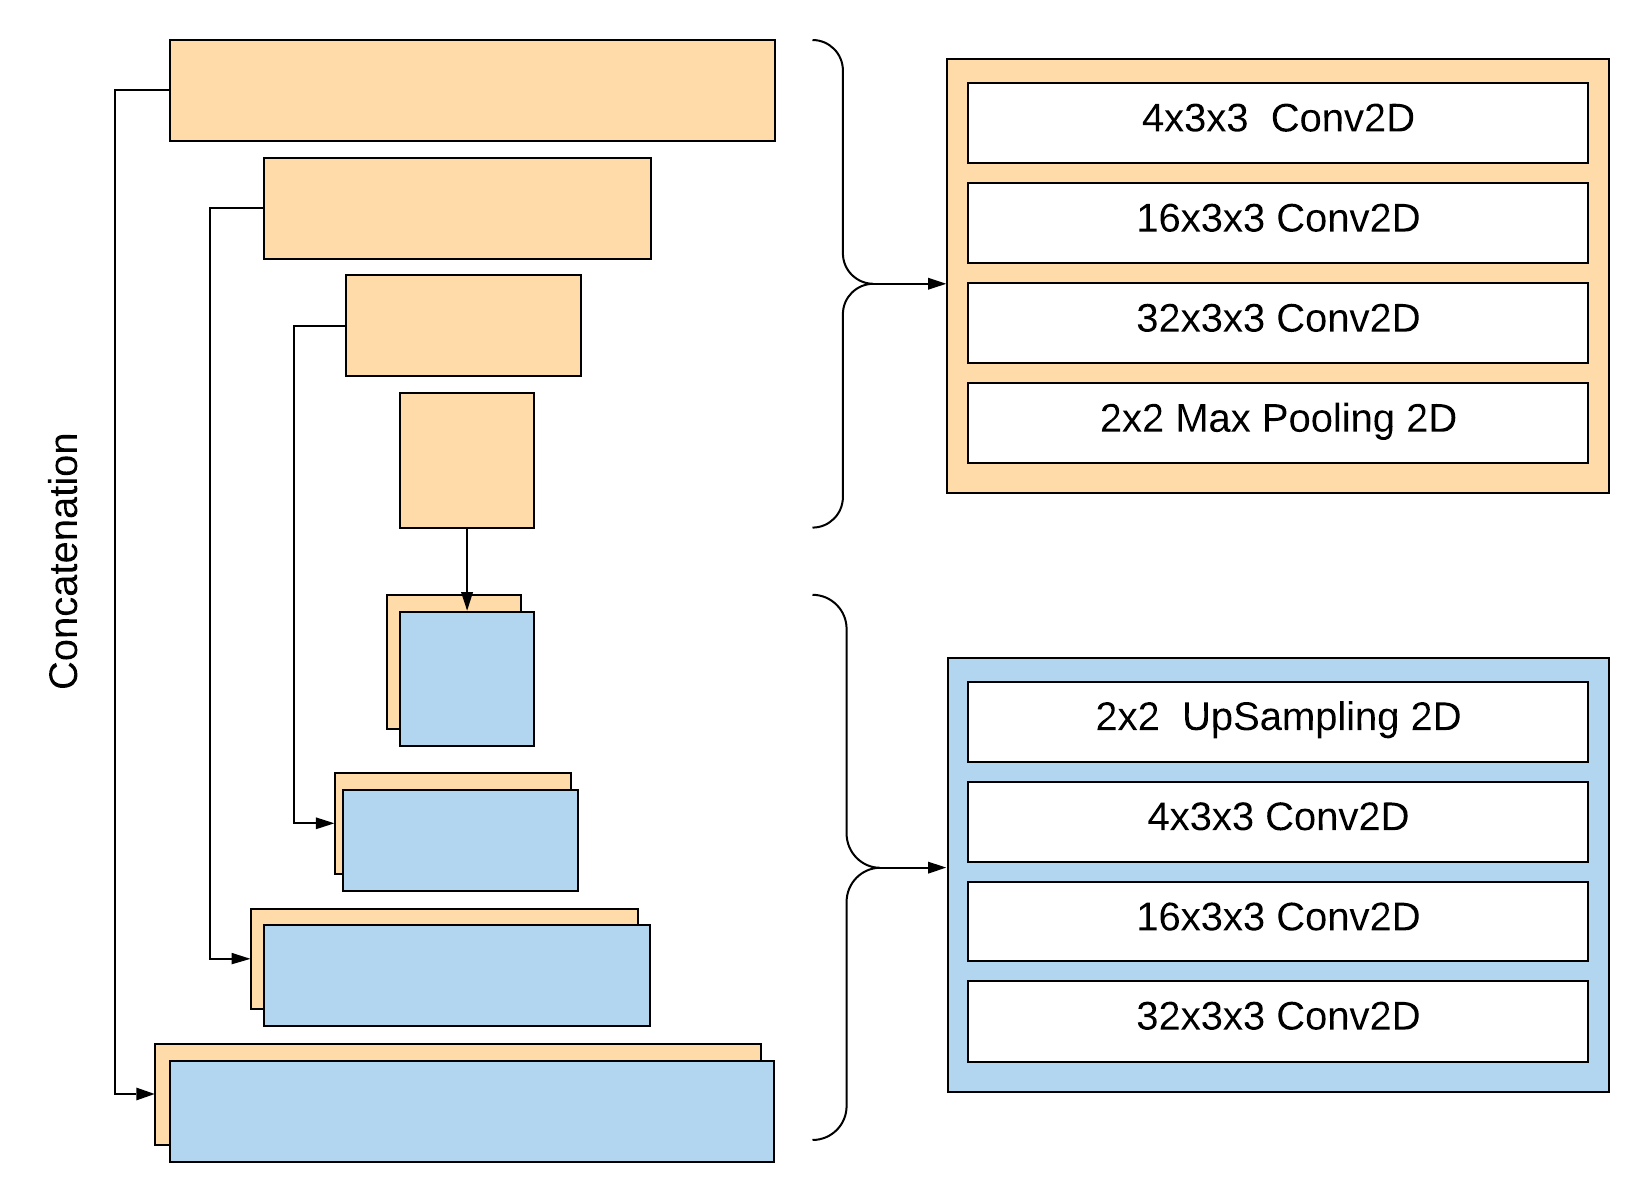
\includegraphics[width = 12cm, height = 10cm]{Figures/A1.png}
    \caption{U-Net architecture (\textbf{A1}). The bottom 4 blue blocks represents the decoder and the above 4 block represents encoder. }
    \label{fig:A1-U-NetArchetecture}
\end{figure}{}

U-Net (\textbf{A1}) architecture as shown in Fig \ref{fig:A1-U-NetArchetecture} is built upon simple idea of using upsampling layer or de-convolution layer  \footnote{not to be confused with the nomenclature, there are various names for de-convolution such as up-sampling layers or transposed convolution layer used by tensorflow and keras (\url{www.tensorflow.org/})} for up scaling the learnt feature and regeneration of depth maps. The motivation for building \textbf{A1} is to evaluate the influence of backbone architecture which has learnt the structural characteristic from a given image as seen before in Section \ref{Chapter3:RelatedWork_NNModel}. Another reason for us to use such approach lies in the simple architecture which is faster to train. The decoder block comprises of transposed 2D convolution layers which have the same dimension as the kernel size of encoder block. This means number of layers in encoder and decoder are the same that's why the name U-Net. 

\textbf{A1} consists of 4 blocks of encoder and decoder part. Each block of encoder consists of 4 layers, 3 layers of 2D Convolutions and 2D max pooling layer of size 2$\times$2 at the end of each block. We designed the 3 convolutions layer with the increasing order of number of filter 4, 16 and 32 with kernel size of 3$\times$3. In the similar way in each decoder block we have 4 layers, starting with an up-sampling layer with kernel size if 2$\times$2 which means the up scaling of the image is in the factor of 2. Nearest neighbor interpolation method used by the up-sampling layer \footnote{\url{www.tensorflow.org/api_docs/python/tf/keras/layers/UpSampling2D}} implemented by keras layer. Towards the end each decoder block has 3 convolution 2D stacked in the similar way as encoder blocks. Each decoder block is concatenated with relative encoder block which has same dimension as shown in fig. \ref{fig:A1-U-NetArchetecture} with arrow marks. The dimension of encoder and decoder block output tensors are kept in same with respect to the width and height if the image input dimension. This can be achieved by having same kernel size of max pooling at encoder part and up sampling layer at decoder, hence the symmetry in the encoder and decoder layers. The last output layer comprises of Convolution 2D layer of 1$\times$1 with sigmoid activation. Also last layer has no stride to keep the dimension same as the input. 
This model has input dimension of (batch size$\times$480$\times$640$\times$3) and output dimension of (480$\times$640$\times$1) for both target RGB image and ground truth depth images. Total trainable parameters of this model is 42,821.



\subsection{Approach 2 (A2) - DenseNet backbone}

\begin{figure}[h]
    \centering
    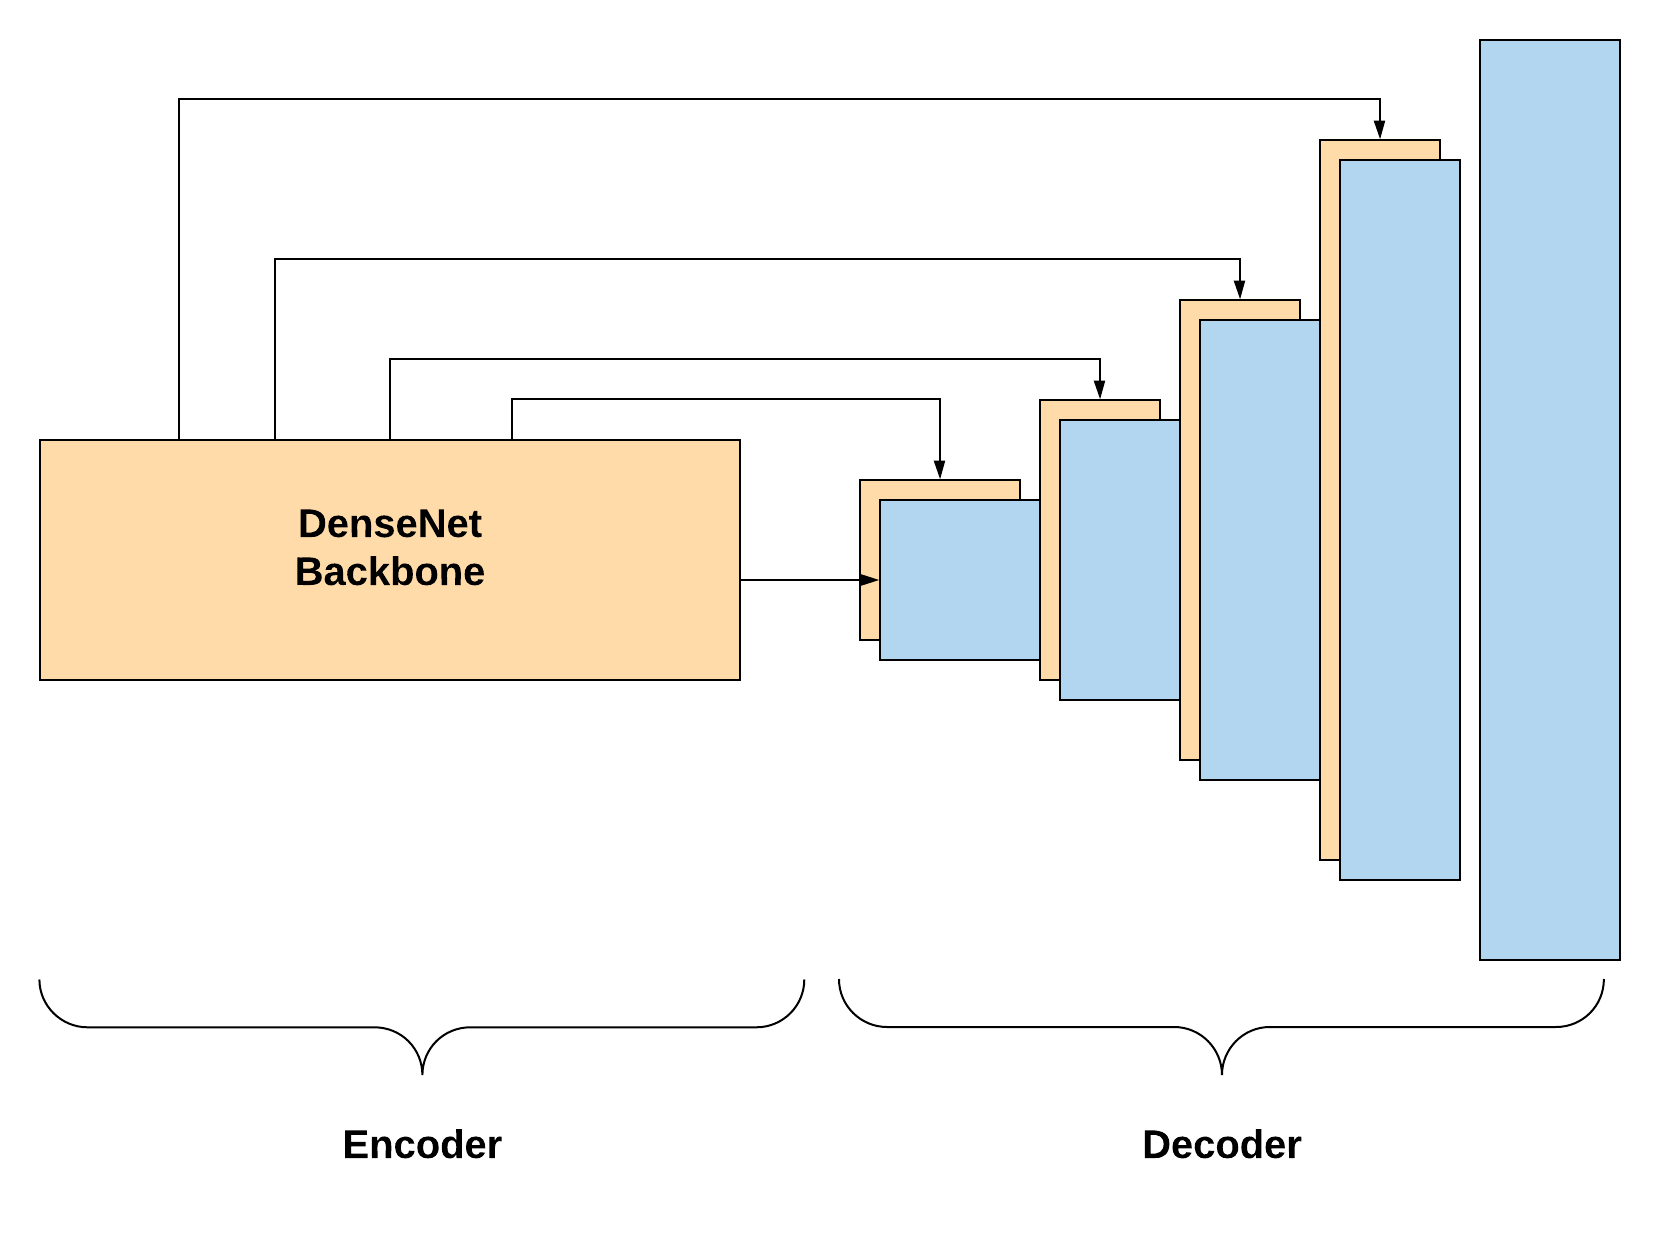
\includegraphics[width = 15cm,  height = 10cm]{Figures/A2.png}
    \caption{\textbf{A2} with DenseNet backbone}
    \label{fig:A2-DenseNet-arch}
\end{figure}{}




As shown in fig. \ref{fig:A2-DenseNet-arch} shows an overview of our second approach \textbf{A2} for depth estimation. We adapted the idea proposed by Alhashim et. al. \cite{Alhashim2018}. The basic idea of this approach \textbf{A2} was to use DenseNet as backbone or as an encoder from our literature study on this topic. The input RGB image is fed to the DenseNet-169 \cite{huang2017densely} network which is pretrained on ImageNet \cite{deng2009imagenet}.  Backbone DenseNet architecture is designed in a feed forward fashion within a dense block or in other words for feed forward design is that each layer is directly connected to every other layer. But since they adapt DenseNet style there is also skip connections between the layers. ImageNet is a large database of images which was build upon WorldNet which is organized in a hierarchical manner, which means the images are trained and clustered according to various classes which give a good hierarchical tree and sub-tree format for classification or clustering. Another great advantage of this net is its versatility of the classes ranging from mammals, vehicles, birds to furniture with 12 subtree which gives us 5247 category at the time of this paper by Deng et. al.\ref{deng2009imagenet}. ImageNet claims to have a order of 50 million images and an average of 5000 image per node \footnote{\url{http://www.image-net.org/}}. ImageNet is also good for object recognition, classification and also clustering problems. Due to such versatility, ImageNet can give us a good generalisation of the physical structure from a 2D image which is very important for our task. This also has proven to give state of the results by the model proposed by Alhashim et. al. \cite{Alhashim2018}. 


The design of this network is in such a way that the output from the DenseNet block is  fed to a successive series of up-sampling layers. The decoder has 5 Bilinear up-sampling blocks. \(4^{th}\) block is designed in a way that it give the output resolution half of its input, which is 230$\times$320$\times$1 for input size of RGB image 460$\times$640$\times$3. The \(5^{th}\) block has up-sampling factor of 2 which gives us full resolution same as input. In all our experiments we use only 4 blocks and in post processing we up sample by the factor 2 to get full resolution. This saves some computational time. The decoder part is trained on the 120,000 images of NYU v2 depth dataset. Also the decoder does not contain any Batch Normalization or other advanced sub multi task layers as seen in the recent state-of-the-art methods in section \ref{Chapter3:RelatedWork_NNModel}.

Each block of decoder comprises of 4 layers, starting with up-sampling by Bi linear with linear interpolation method. followed by concatenation operation and 2 convolutions 2D layers. The number of filters for these convolutions layer is decided by the number of filter obtained from the encoder layer which can be given by \(D_n =  {E_m} / {2^n}\) where \(D_n\) is number of filters at decoder block \(n\) and \(E_m\) is the number of filter present in the layer which is concatenated from encoder. The kernel size of these two convectional layers are of size (3$\times$3). The model proposed by  \cite{Alhashim2018} has target input dimension of 460$\times$640$\times$3 for RGB image and  dimension of 230$\times$320$\times$1 for ground truth label and we acquire the same principles for all our experiments. Also in the results section \ref{Chapter6:Results} we had some experiments by retraining the decoder part with different dataset and configurations to understand the influence of different. Total trainable parameters of this model is 42,657,689.



\section{Structure Depth Dataset Overview} 
\label{Chapter4:Dataset} 

Our aim in this work is to deliver a robust system for depth prediction as seen in the Figure \ref{fig:Proposed_Model} for a portable hand held mobile device. In our case it is an IPad integrated with Structure sensor. In order minimize the difference between the predicted depth maps and depth map generated from Structure sensor we need to train with the similar dataset. We have also validated this in our experiments which will be discussed below in Section \ref{Chapter6:Results}. As discussed in the Section \ref{Chapeter1:Topic_Description}, this will also help us to study the effect of different camera and sensor properties on different environment.\\

As we have seen earlier in Chapter \ref{Chapter3:RelatedWork}, there are multiple datasets available but almost none fit our context. As we are already exploiting the depth features from NYU V2 for general prediction, we would like to produce a dataset which is solely application based. Here our application is mobile device, particularly IOS, we generate the dataset using an IPad. This will not only make the intrinsic parameters to be learned by the network but also particularize for IOS based devices. As we use IPad as integration, all the RGB Images are received from the IPad's camera. The features we want the neural network to learn and predict should have the same camera intrinsic parameters in order to decrease the amount of pre processing of the dataset. Hence, We first calibrate IPad with Structure Sensor before collecting the Dataset. Another major advantage of using Structure Sensor with an IPad over Kinect is the resolution of RGB and Depth Images. While Kinect V2 has $512\times424$ Infrared camera resolution, Structure Sensor can go upto $640\times480$. \\

Our Dataset consist of two versions. The first version(SD\_V1) which was taken during the training of \textbf{A1} network which is detailed in Section \ref{Chapter5:Methodology}. In SD\_V1, we produced no hole depth images with wall of threshold 4 m. Since the temporal resolution of Structure Sensor is as high as 60 fps, there is not much difference in frames. So, in order to achieve a quality dataset, we saved a frame in every 10\textsuperscript{th} frame. Having a 60 fps video stream, we saved 6 fps. This removes redundant data and prevents us from overfitting. In the second version(SD\_V1) of our dataset, we captured every 2\textsuperscript{nd} frame per second giving us a temporal resolution of 30 fps. In SD\_V1, we removed the distance threshold and filled it with holes instead. We trained \textbf{A2} network with the new dataset. Including SD\_V1, we have a total of 18 scenes and consisting of 2675 images captured using an Apple iPad Pro version 12.9 (2015) model and a Structure Sensor only. The dataset majorly includes images from office and classrooms environments. It consist of RGB Images of $640\times480$ as 3 channel $\times$ 8 bit int and Raw Depth Images of 640 $\times$ 480 as 1 channel. Both of the images are saved using lossless compression. Later, we also perform some processing to synchronize RGB and depth images and to fill the holes of depth image which will be discussed later in this chapter. We also provide the camera extrinsic parameters as a numpy matrix of $4\times4$ which is useful for reconstruction of a scenario.\\



\subsection{Technical Specification of Structure Sensor}
The Structure Sensor \footnote{\url{https://structure.io/}} is a 3D scanner introduced by Occipital in 2014. As the name suggests, it uses Structured-Light-System (SLS) 3D scanning\cite{Kalantari}. It can be easily attached to an IPad and with Structure SDK it enables us to generate good quality RGB image stream from IPad and its realtive depth stream from Structure Sensor at the simultaneously. As it only weighs 95 grams and can be used as an extension to mobile device, it makes the sensor very portable. With possibility of recording 60 frames per second at a resolution of $640\times480$\cite{Kalantari}. When compared to Kinect V2, it has more depth image resolution. The comparison can be seen in table \ref{table:KinectVsStructureSensor}. The minimum range it can capture is 40 cm while it can capture till 4 m with fine precision. After 4 m the precision is not satisfactory enough to use it for the dataset. Occipital claims it has low frame-to-frame noise and provides 100\% fill rate on most of the materials. On the other hand IPad Pro 12.9 provides us with an RGB video stream of $1920\times1080$ at 30 frames per second and $1080\times720$ at 60 frames per second. IPad Pro also provides us with Camera extrinsic parameters which are useful for the reconstruction of the scenario.\\

\begin{table}[h]
\begin{tabular}{@{}lll@{}}
\toprule
\textbf{Features}                    & \textbf{Kinect V2}           & \textbf{Structure Sensor}         \\ \midrule
Depth Sensor Type           & ToF & SLS                 \\
RGB Camera Resolution       & $1920\times1080$, 30 fps & $1920\times1080$, 60 fps     \\
IR Camera Resolution        & $512\times424$, 30 fps   & $640\times480$, 60 fps                 \\ 
Field of View of IR Camera  & $70^\circ\times60^\circ$           & $58^\circ\times45^\circ$                         \\
Recommended Operative Range & 0.4 m - 3.5 m       & 0.4 m - 3.5 m                                  \\
           &                     & 
\end{tabular}
\caption{Comparison of Kinect V2 and Structure Sensor}
\label{table:KinectVsStructureSensor}
\end{table}

\begin{figure}[h]
    \centering
    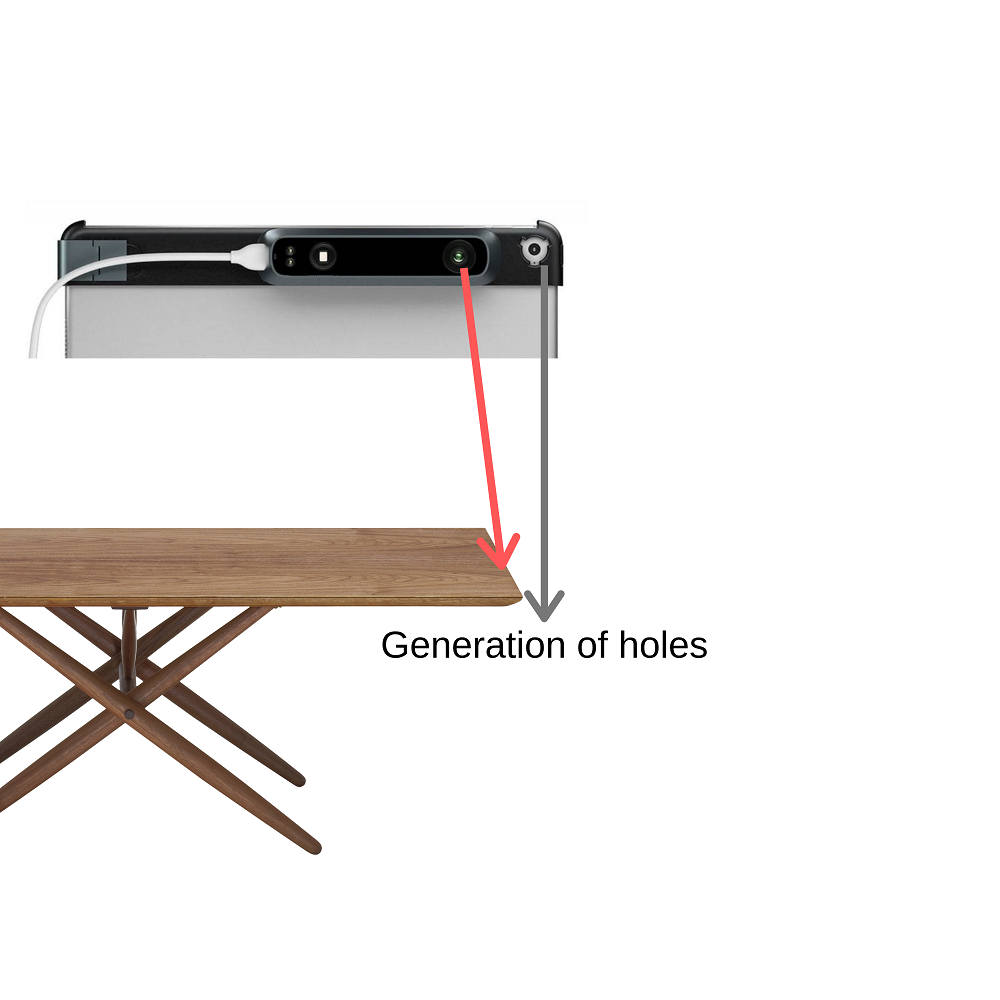
\includegraphics[scale=0.4]{Figures/holes.png}
    \caption{Generation of holes due to parallax}
    \label{fig:holes}
\end{figure}
While these sensors are great devices they have some limitations. The distance they can measure is limited and they suffer from reflection problems on transparent, shiny or very matte and absorbing objects. Another limitation is holes generated by parallax effect happening due to difference in position of the camera of IPad and Structure Sensor\cite{Kalantari}. In simpler terms, it works like human eyes. If we look at an object using only either of our eyes, we could notice disparities. When there is an object we try to focus on, our eyes which located at different position like the sensors in the Structure Sensor, they will see the object from different angles. If the object is close enough, then sometimes one eye can see what is behind and other can not. This can be seen in figure \ref{fig:holes}. As a result, it produces a shadow of holes which can be seen in figure \ref{fig:holes2}.



\begin{figure}[!]
\centering
    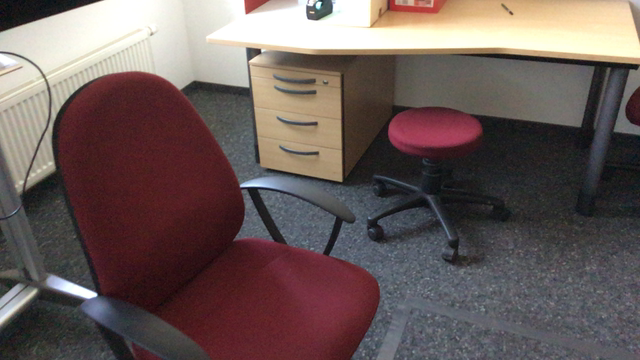
\includegraphics[scale=0.29]{Figures/RGB.png} 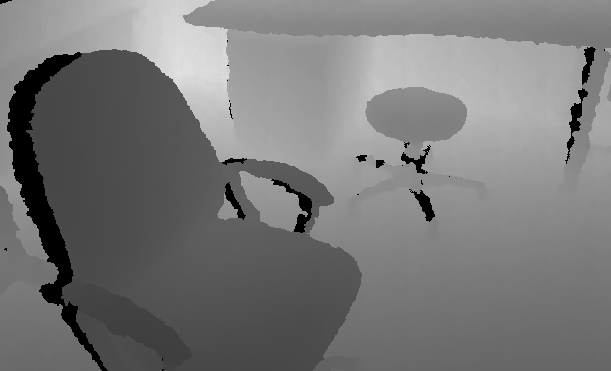
\includegraphics[scale=0.37]{Figures/Depth.png}
    \caption{Holes produced in depth image}
    \label{fig:holes2}
\end{figure}


\subsection{Dataset Collection}

A significant role in Machine Learning is played by Dataset and the collection of it makes most influence on the features that network learns. As the distance is limited in Structure Sensor and due to our scope of research we focus on indoor offices and classrooms environments. While capturing the dataset, one should keep in mind that the network should learn only the novel features not the artifacts. One good instance of this would be capturing the depth of a screen. Since, a screen has reflective black surface, it loses depth information resulting holes in depth image as seen in Figure \ref{fig:screens}. If we feed these images to the network, it might learn the features such as, screen is always at, let say x distance, where x is pixel value we assign to such holes. These holes are the undesired features and called artifacts. Such artifacts could be produced due to various reasons. It could be the reflective/absorbing nature of the surface of an object or the distance and position of the object\cite{geomar41830}. As a reflective/glossy surface leads us to wrong or no generation of depth pixel, we try to avoid them while capturing. Figure \ref{fig:screens} is one good example of such holes. As we notice in the RGB image there are two screens, one is predicted in some regions while other one is totally lost. In indoor environments, such objects are inevitable. Thus, in such problems we use techniques like inpainting \cite{inpainting}. Image inpainting could also be used to resolve artifacts due to parallax effect discussed in section previous section.\\
\begin{figure}[h]
    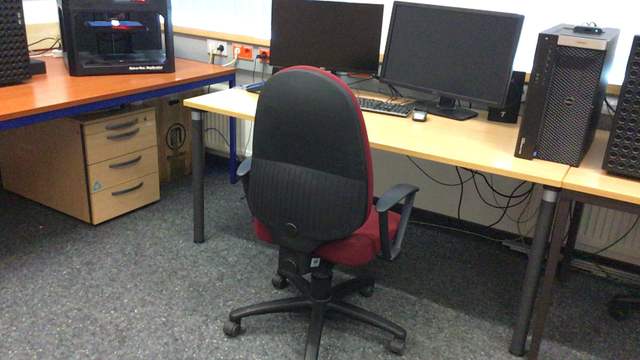
\includegraphics[scale=0.29]{Figures/7.png} 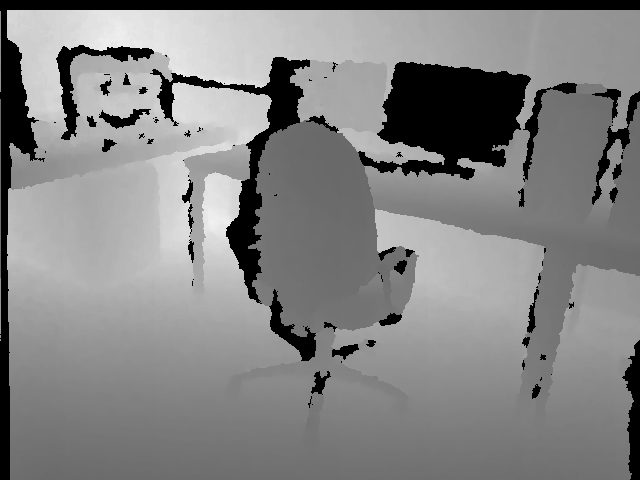
\includegraphics[scale=0.24]{Figures/Raw7.png}
    \caption{Holes produced in depth image due to reflectivity of the screen}
    \label{fig:screens}
\end{figure}
 

Since, the accuracy decreases with the increase in depth \cite{deptherror} and because the recommended range is no more than 4 metres(m) for Structure Sensor \cite{Kalantari}, we remove all the pixels which are far away than 4 m. These pixels can be resolved using further predictions and post processing. This also protects our network from learning the artifact of distant objects as a wall as discussed in \ref{Chapeter1:Topic_Description}.\\

\subsection{Data Processing}

The very first step of processing the dataset would be registering the depth pixels. After we have calibrated the camera, we convert the pixels received from Structure Sensor to millimetres(mm) for ease of understanding as the pixel value have a non linear relationship. After we have the distances in metres, we want to eliminate all the possible artifacts as these images still contain holes and precision less pixels. Usually, far away pixels have less precision and results in holes as well\cite{deptherror}. It is a good idea to conserve those pixels as holes in order to reconstruct the environment by later predicting the future frames. Firstly, after we have the Depth images in metres, we save all the holes by its pixel position or index for all the pixels more than 4000 mm so that we can use that information later. By doing so, we can eliminate the distance threshold artifact discussed earlier.

\begin{figure}[!]
    \centering
    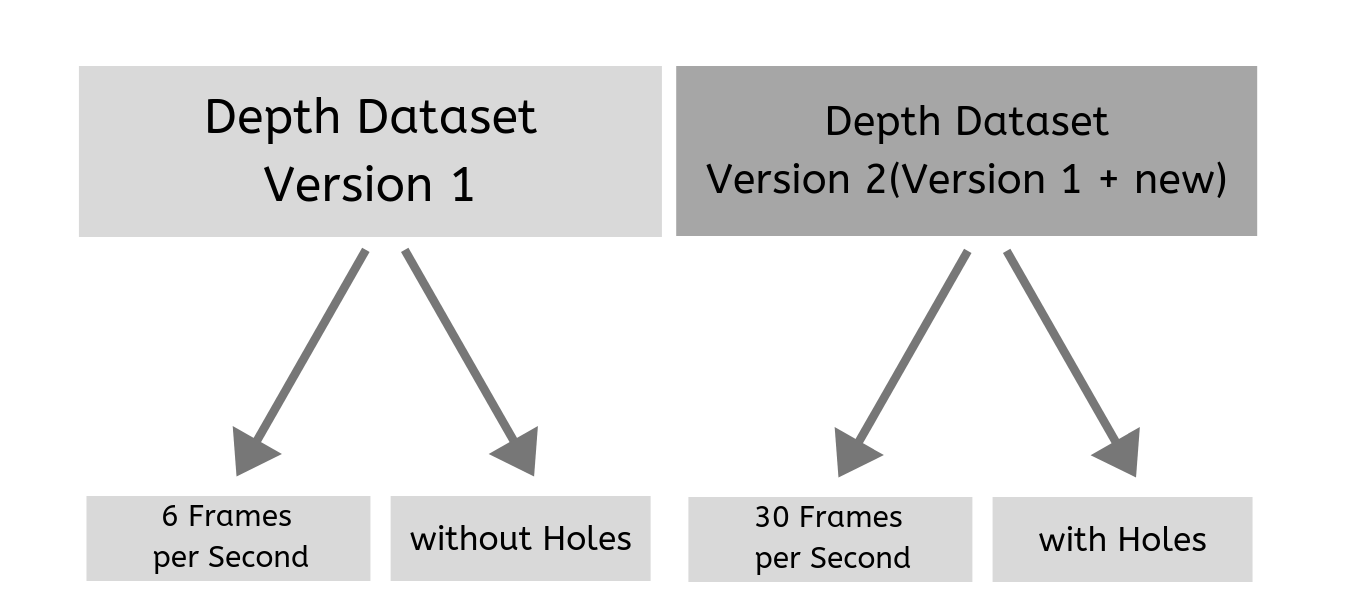
\includegraphics[scale=0.35]{Figures/versions.png}
    \caption{Versions of our proposed dataset}
    \label{fig:datasetversion}
\end{figure}

\begin{figure}[h]
    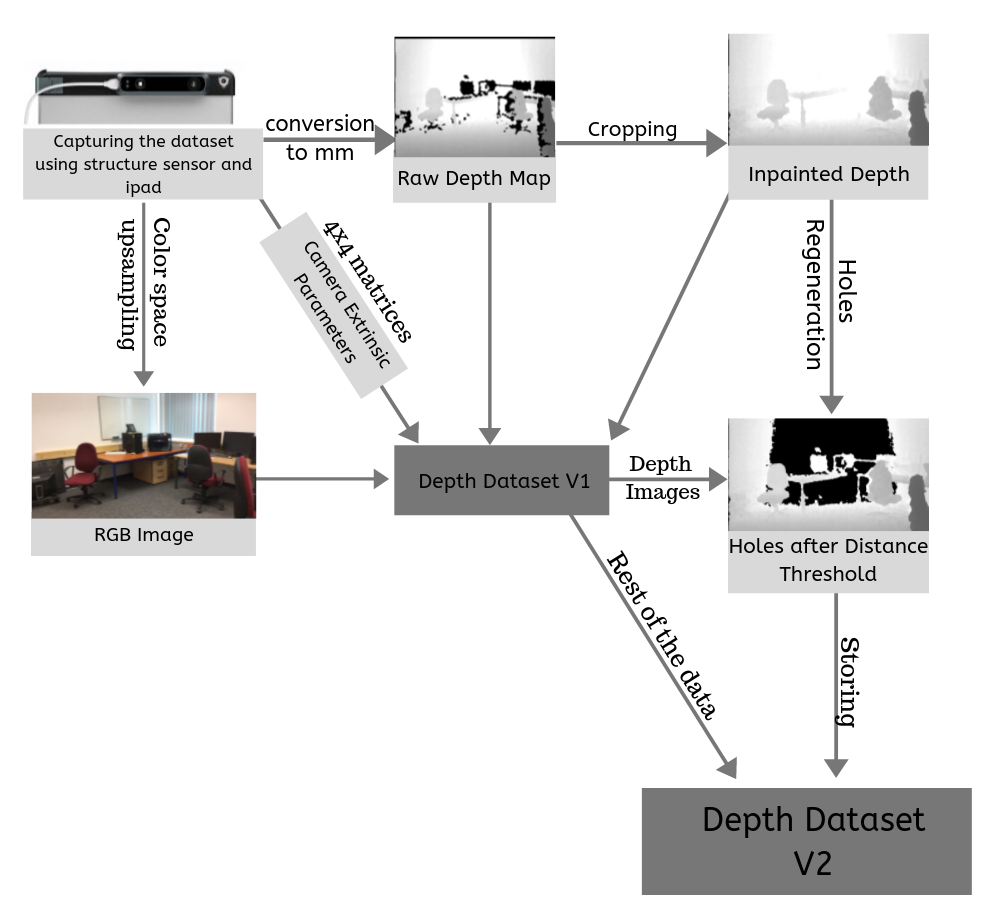
\includegraphics[scale=0.50]{Figures/process.png}
    \caption{Different stages of processing the depth frames}
    \label{fig:processing}
\end{figure}

As discussed earlier, the Depth images contains holes from shiny/glossy objects\cite{shiny}. In office environments, these holes are mostly generated by Computer Displays. Since we do not want our network to learn that all the screens are close(0 pixel), we interpolate these holes. We do this by inpainting \cite{inpainting} the whole image. This fixes the issues of shadows produced due to the parallax as well. Noting that it inpaints the pixels more than 4 m too. SD\_V1 of our dataset consisted of depth images which were totally inpainted and there were no holes as can be seen in \ref{fig:datasetversion}. Basically which means, if some of the pixels which are far away than 4 m are missing, they are interpolated using nearest neighbours. As we know, these predictions are not very accurate from past discussion, it is also possible that the inpainted depth is not correct. So In SD\_V1, successor of SD\_V1, we use the index of pixels of depth more than 4 m we saved now later in the process. This will reproduce all the holes which were more than 4 m as missing information is better than wrong predictions. These holes can later be predicted using the future frames. Our depth image is now ready to be fed to the network but as one would have noticed before, The size of the Color Image and Depth Image does not match since they have different aspect ratios due to different camera sources. So, In the end we crop the depth image centre focused in order to make them compatible with the network. We can understand this through Figure \ref{fig:processing}, where we show how the captured data and is processed and stored. \\



\newpage
\section{System Setup}
\label{Chapter5:Experimental_Setup}
\subsection{Training and Experimental Configurations}

 Our entire experimental experimental configuration are described in the fig \ref{fig:Experimental_Setup}. All the configuration where made based on two model \textbf{A1} and \textbf{A2} and two data pre-processing \textbf{Holes} and \textbf{No\_Holes}. Added to this we also did a \textbf{transfer learning} over \textbf{A2} by retraining the model with Structure Sensor dataset. This gives two models and five different configuration to analyze foe our study. 


First, Our proposed model \textbf{A1} is a simple U-Net style architecture - also can be categorized as encoder-decoder style of architecture. There are two specific reason for designing simple architecture. (a) To understand if a simple network can learn the feature from a given depth image. one of the advantage of a simple small network is we have faster computation for the implementation (b) If a new architecture can learn without any prior knowledge of such structures, if yes how well can it perform. This motivated us to evaluate our model performance against an existing model.As previously discussed in the Chapter \ref{Chapter3:RelatedWork}  where chose approach \textbf{A2} proposed by Alhashim et. al. \cite{Alhashim2018}. Also developing \textbf{A1} involved various network configuration parameter optimization only the final best working model has been documented in the Section \ref{Chapter5:A1}. \\

Secondly, we wanted to investigate if dataset from different sensor with different cameras intrinsic and extrinsic properties can influence our results.  This result was necessary because our study is to answer if we can replace structure sensor by neural network, thus we have structure dataset to get as close results as structure sensor. This experiment also gives us a good validation base if there is a need for task and hardware based dataset for neural network models to perform on cross platform environment - in our case  the cross platform environment would be between neural network trained kinect dataset and mimicking Structure Sensor. For this our idea was to train our model with two dataset NYU\_v2 depth dataset and structure depth dataset. We train only the decoder block of \textbf{A2}. Alhashim et. al \cite{Alhashim2018} model was trained on 120,000 images from NYU\_v2 dataset and these weights for decoder block was publicly available. Therefore we call this experiment setup as \textbf{Transfer Leaning} approach. Hence we had two experiments, one by evaluation the model trained on  datasets from kinect sensor and another trained on both kinect and structure. By using the pre-trained weights, it saves computational time and memory while different training and experimental configuration. \\

Thirdly, we wanted to investigate if a model can learn the holes generated from the SLS sensor. In our literature study in Section \ref{Chapter3:RelatedWork} most of the work where based on approach where the depth data was processed  in a way where the holes where interpolated. The most common and widely used method was to either in-paint (or fill) the holes using neighboring pixel \cite{silberman11indoor} method. We approached this problem by saving the holes and map all the invalid holes to zero value instead of finding neighboring pixel which was used in NYU dataset. We trained \textbf{A2} model in two different fashion. One by mapping the holes to a zero value we call it as \textbf{A2\_Holes} and another we find the neighboring pixels and we call this approach as \textbf{A2\_NoHoles}.

\begin{figure}[h]
    \centering
    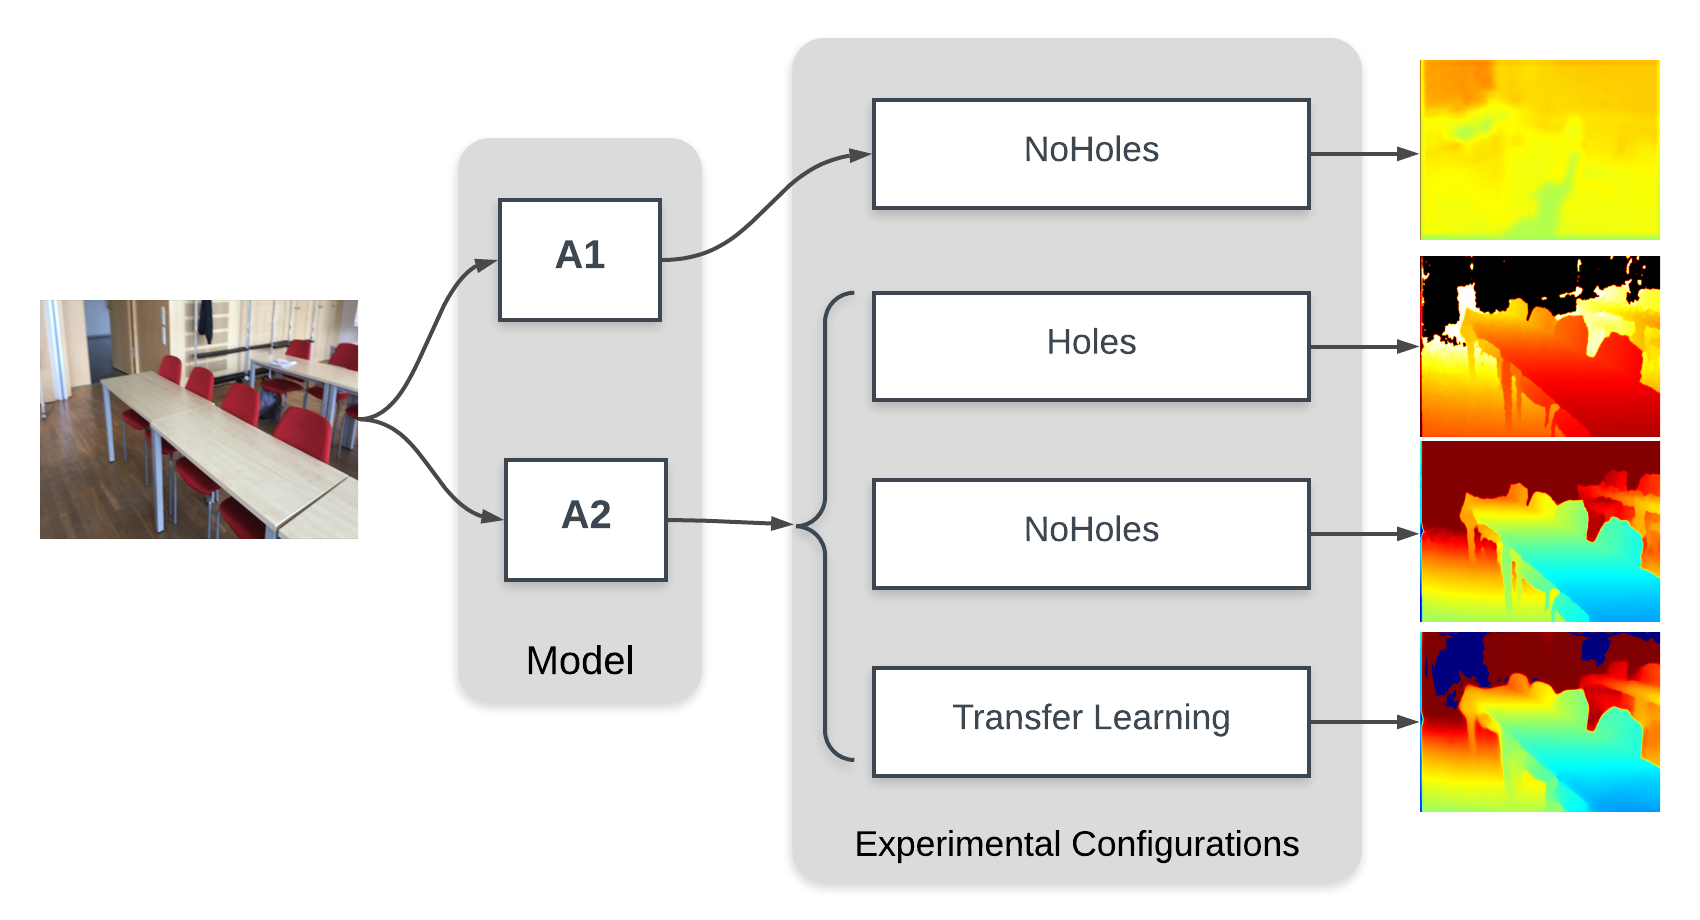
\includegraphics[width = 14cm]{Figures/config_setup.png}
    \caption{Different experimental configuration were setup based on \textbf{A1} and \textbf{A2} approaches}
    \label{fig:Experimental_Setup}
\end{figure}{}

Finally, we wanted to investigate the best working configuration to evaluate against a baseline model on the test set of Structure Sensor. 

Therefore in summary, we have two model \textbf{A1} and \textbf{A2} for validating the proposed model and effects of structural Characteristic. Further more \textbf{A2} model where retrained with two different modified input features for investigating on regeneration of holes. This gives us two more configuration of \textbf{A2} model namely \textbf{A2\_Holes} and \textbf{A2\_NoHoles}. These four configuration where made to fit the three different experimental conditions. First experiment is based on changing parameters with respect to encoder. second experiment is based on changing parameters at decoder. Third is by evaluating against two dataset configurations.

\subsection{Loss Function}
\label{Chapter5:LossFunction}
A standard loss function for depth estimation problems is computed by finding the difference in predicted values \(\hat{y}\) and truth \(y\). In our work we use loss function proposed by \cite{Alhashim2018}. One of the significe of this loss function is, it not only computes difference in t \(\hat{y}\) and truth \(y\) acting as minimizing error function but also it focus on higher frequency penalizing. The reason for having weight for higher frequency of an image is to compute the performance of the network corresponding to the object boundaries. The resultant loss function \(L\) is computed as a weighted sum of three loss functions which are pair wise loss \(L_{depth}\), image gradient loss \(L_{grad}\) and structure similarity loss  \(L_{SSIM}\) which is given by:


\begin{equation} \label{eq:loss}
       L(y, \hat{y}) = \lambda_{1} L_{depth}(y, \hat{y}) + \lambda_{2} L_{grad}(y, \hat{y}) + \lambda_{3} L_{SSIM}(y, \hat{y})
\end{equation}




%%%%%%%%%%%%%%%%%%%%%%%%%%%%%%%%%%%%%%%%%%


%\begin{itemize}
 %   \item First the pare wise depth is given by:
%\end{itemize}{}
\begin{equation} \label{eq:loss_depth}
      L_{depth}(y, \hat{y})= \frac{1}{n} \sum_{p}^{n} \left|y_{p} - \hat{y}_{p} \right|
\end{equation}

First the pare wise depth is given by euation \ref{eq:loss_depth}. This gives us a pixel level understanding of error between ground truth and predicted image.  
%%%%%%%%%%%%%%%%%%%%%%%%%%%%%%%%%%%%%%%%%%

%\begin{itemize}
%    \item Structure similarity loss
%\end{itemize}{}
\begin{equation} \label{eq:loss_grad}
       L_{grad}(y, \hat{y}) =  \frac{1}{n} \sum_{p}^{n} \left| g_{x} (y_{p} - \hat{y}_{p}) \right| + \left| g_{y} (y_{p} - \hat{y}_{p}) \right|
\end{equation}


Secound, the \(L_{grad}\), which computes the gradient changes with respect to its neighboring pixels. Here the image gradient \(g\) is computed in two directions \(g_{x}\) and \(g_{y}\) which compute the differences in \(x\) and \(y\) component of the depth images. \\


\begin{equation} \label{eq:loss_SSIM}
       L_{SSIM}(y, \hat{y}) = \frac{1- SSIM(y, \hat{y})}{2}
\end{equation}

Third, the Structrural Similarity Index (SSIM) proposed by Wang et. al. \cite{wang2004image} gives us a good understating of groups of pixel based of comparative measure of three components individually which are luminance, contrast and structure similarities between ground truth and predicted. The final \(L_{SSIM}\) is a reciprocal version of SSIM as in \cite{Alhashim2018,  ummenhofer2017demon, huang2018deepmvs}.
%%%%%%%%%%%%%%%%%%%%%%%%%%%%%%%%%%%%%%%%%%


%\begin{itemize}
%    \item Image gradient loss:
%\end{itemize}{}


We used tensorflow implementation of \(L_{grad}\) \footnote{\url{https://www.tensorflow.org/api_docs/python/tf/image/image_gradients}} and \(L_{SSIM}\) \footnote{\url{https://www.tensorflow.org/api_docs/python/tf/image/ssim}}  in our study \cite{tensorflow2015-whitepaper}. Though out the experiments the weightage factor for our loss function in equation \ref{eq:loss} where set to  \(\lambda_{1} = 0.1, \lambda_{2} = 1, \lambda_{3} = 1\) suggested by \cite{Alhashim2018}. Hence we try to supervise our network based on structural similarities more than pixel level similarities. 


\newpage

%From the above equation \ref{eq:loss} The 

\subsection{Evaluation Metrics}
\label{Chapter5:Evaluation_mat}
For our evaluation we use standard metrics used in prior work \cite{Alhashim2018, eigen2014depth}. The error metrics are defined as follows:
%%%%%%%%%%%%%%%%%%%%%%%%%%%%%%%%%%%%%
\begin{itemize}
    
    \item Root Mean Squared Error (RMSE):
    
\end{itemize}{}

\begin{equation} \label{RMSE}
        \sqrt{\frac{1}{n} \sum_{p}^{n}{(y_{p} - \hat{y}_{p}})^2}
\end{equation}
%%%%%%%%%%%%%%%%%%%%

\begin{itemize}

    \item Average (${log_{10}}$) error: 
    
\end{itemize}{}

\begin{equation} \label{avg_log}
    \frac{1}{n} \sum_{p}^{n} \left|log_{10}(y_{p}) - log_{10}(\hat{y}_{p}) \right|
\end{equation}

%%%%%%%%%%%%%%%%%%%%%%%%%%%%%%%%%%%%%%

\begin{itemize}
    \item Threshold Accuracy (\(\delta_{i}\)): 
\end{itemize}{}

\begin{equation} \label{ThresholdAcc}
    {\delta = max (\frac{{y_{p}}}{\hat{y_{p}}}, \frac{\hat{y_{p}}}{{y_{p}}})}
\end{equation}

The threshold accuracy is computed based on 3 different threshold values which are given by \(\delta < a_{i}\)  \(a_{1}= 1.25^1, a_{2} = 1.25^2, a_{i} = 1.25^3\)  
%%%%%%%%%%%%%%%%%%%%%%%%%%%%%%%%






\subsection{Implementation Details}
\label{Chapter5:HardwarSoftwareDetails}
%ECCRTX-OPS 84T 
Here we mention all the necessary tools and modules used in this study. 

 \subsubsection{Training Configurations} 
 \label{Chapter4:TrainConfigurations_i}

 Though out all our  experiments we trained all our model for 1000 epoc with an early stopping of 10. We used Adam \cite{kingma2014adam} optimizer with the learning rate of \(10^{-4}\). For loss function and evaluation metrics we use methods as described in Section \ref{Chapter5:LossFunction} and Section \ref{Chapter5:Evaluation_mat} respectively.
 
 \subsubsection{Dataset} 
  \label{Chapter4:DatasetForsplits-i}

 We used two dataset they are NYU\_v2 and and two versions of Structure depth dataset (SD\_v1 and SD\_v2) datasets. NYU\_v2 is publicly available and SD\_v1 and SD\_v2 where creatre for this task. For all the experiments we used 80-10-10 (\%) split for training, validation and test set. We had one test sets for each of the dataset. For NYU\_v2 we used standard test set available online comprising of 1449 RGBD images. Similarly for SD dataset we used 
 
 
\subsubsection{Hardware:} 
\label{Chapter4:Hardware_i}
For all our experiments we used \textit{Nvidia Quadro RTX 8000} graphic card with Graphics processor GDDR6  having memory of 48 Gigabyte on Linux operating system with Ubuntu distribution 18.04. For capturing dataset, we used Apple iPad Pro version 12.9 (2015) integrated with Structure Sensor by Occipital with the help of Structure Software Development Kit.


\subsubsection{Software} 
\label{Chapter4:Software_i}
For the implementation of Neural Network model and related tasks, we used Keras 2.2.4 framework with Tensorflow 1.13.1  backend for python environment \cite{tensorflow2015-whitepaper}. CUDA 10.1 (a software layer which gives direct access for multiple processing on GPUs having two main key attribute of hierarchical multiprocessing thread groups and shared memory \cite{nickolls2008scalable}) the GPU  the above mentioned  \textit{Nvidia Quadro RTX 8000} graphic card  Additionally, we used openCV library \cite{opencv_library} for varous image processing tasks. For dataset collection, we used Xcode 10.2 \footnote{\url{https://developer.apple.com/documentation/xcode_release_notes/xcode_10_2_release_notes}} to send the data over the network.



\newpage



\section{Schedule and Milestones}
\begin{figure}[h]
\centering
    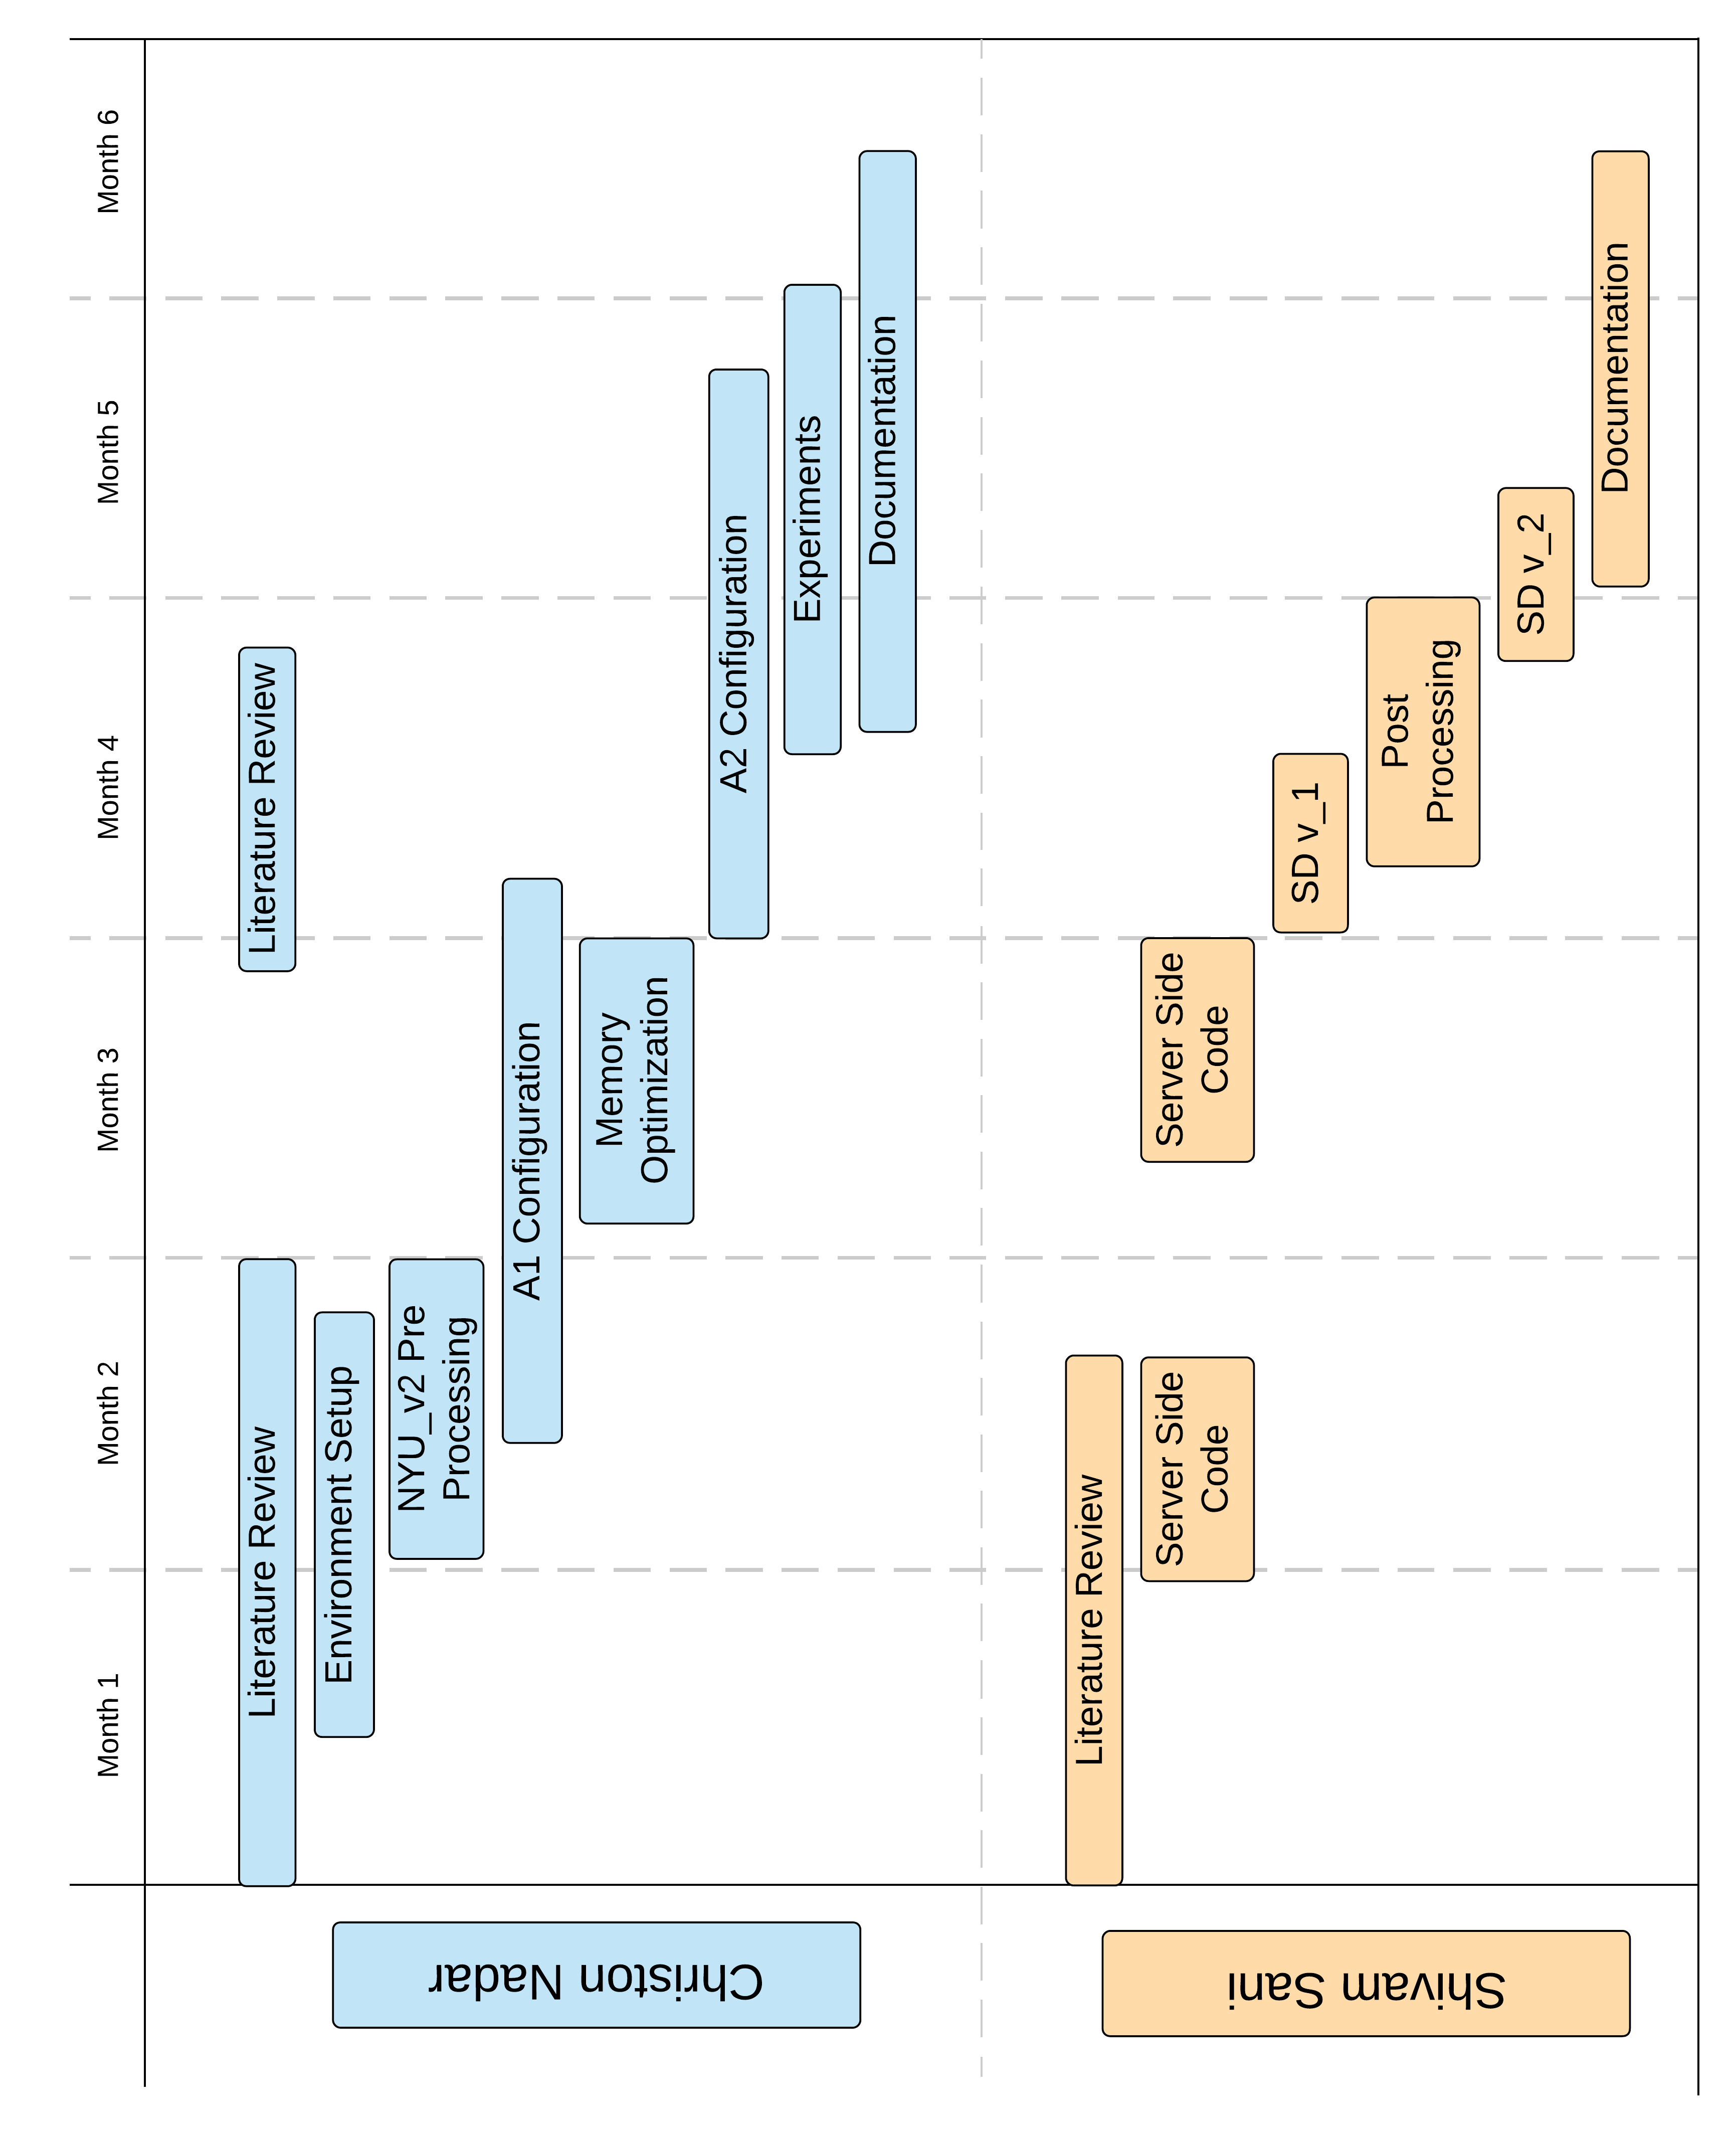
\includegraphics[width=14cm, height=18cm]{Figures/ganntL2.png}
 \caption{Gannt Diagram}
    \label{fig:Gannt_Dia}
\end{figure}
\newpage

 
% Chapter Template


\chapter{Results and Discussion}

\label{Chapter6:Results}

%----------------------------------------------------------------------------------------
% Transfer learning
% effect of loss function
% effect of camera intrinsic 
% effect of Hyper parameter
% Effect of recreating holes.. 
 
 
%----------------------------------------------------------------------------------------
In this chapter we have evaluated your system and presented a comparative results  based on different experimental setup discussed in section \ref{Chapter5:Methodology}. We have categorized our experiments into 3 different sections as shown in the table below \ref{table:Results_main} to investigate in three difference areas. This table lists all the experiments carried out for this study on depth estimation. In the following sections we will be describing our results mentioned in the table and will be discussing about it in its respective sections.  We have 3 accuracy values based on different threshold namely (a1, a2, and a2) and two error metrics namely root mean square error (rms) and log\_10 error as mentioned in section. Experiments \textbf{E1} and \textbf{E2} where performed to understand the importance of structural dependency of depth maps and to test our proposed model against the state of the art system. In experiments \textbf{E3} and \textbf{E4} we validate the influence of different camera intrinsic properties over data from structure sensor, by this we can also see the influence of transfer learning even when trained on different dataset with different feature properties. Experiments \textbf{E5} and \textbf{E6} was carried out to study behaviour of probabilistic distribution over the invalid pixel which we call it as holes, this leads us to answer the question of efficient way for depth estimation.

 
% Please add the following required packages to your document preamble:
% \usepackage{multirow}
\begin{table}[h]
\begin{tabular}{p{0.05\linewidth}p{0.3\linewidth}p{0.1\linewidth}p{0.1\linewidth}p{0.08\linewidth}p{0.08\linewidth}p{0.07\linewidth}}
\hline
\textbf{\#} & \textbf{Model} & \multicolumn{3}{l}{\textbf{Accuracy}} & \multicolumn{2}{l}{\textbf{Error}} \\ \cline{3-7} 
                    &                        & a1       & a2       & a3      & RMSE         & log\_10      \\ \hline
\multicolumn{7}{l}{\texttt{Influence of Structural Characteristics}}                                            \\ \hline
\textbf{E1}                  &  \textbf{A1}  & 0.22         & 0.43          &  0.61       & 0.34            &   0.001           \\ \hline
\textbf{E2}                  & \textbf{A2}  &    0.60  & 0.859 & 0.93       &   0.19          &0.11              \\ \hline
\multicolumn{7}{l}{\texttt{Influence Of Transfer Learning}}                                                                   \\ \hline
\textbf{E3}                  & \textbf{A2\_Holes}(N+S)              & 0.39   & 0.58   & 0.65  & 0.27      & 1.70       \\ \hline
\textbf{E4}                  & \textbf{A2\_Holes}(S) & 0.33   & 0.55   & 0.63  & 0.34      & 1.78       \\ \hline
\multicolumn{7}{l}{\texttt{Holes Regeneration}}                                                       \\ \hline
\textbf{E5}                  & \textbf{A2\_NoHoles}            & 0.98   & 0.98   & 0.98  & 0.10       & 0.18        \\ \hline
\textbf{E6}                  & \textbf{A2\_Holes}              & 0.39   & 0.58   & 0.65  & 0.27      & 1.70       \\ \hline
\end{tabular}

\caption{This table list all the results of experimental configuration performed. These experiments are grouped in to three categories. In E3, (N+S) denotes that model trained on NYU\_v2 and SD, where as in E4, (S) denotes model trained on SD\V2}
\label{table:Results_main}
\end{table}

\newpage

\section{Influence of Structural Characteristics}
 \begin{figure}[h]
\settoheight{\tempdima}{\includegraphics[width=.32\linewidth]{example-image-a}}%
\centering\begin{tabular}{@{}c@{ }c@{ }c@{ }c@{}}
&\textbf{RGB} & \textbf{Truth} & \textbf{Predticted} \\
\rowname{E1 (a)}&
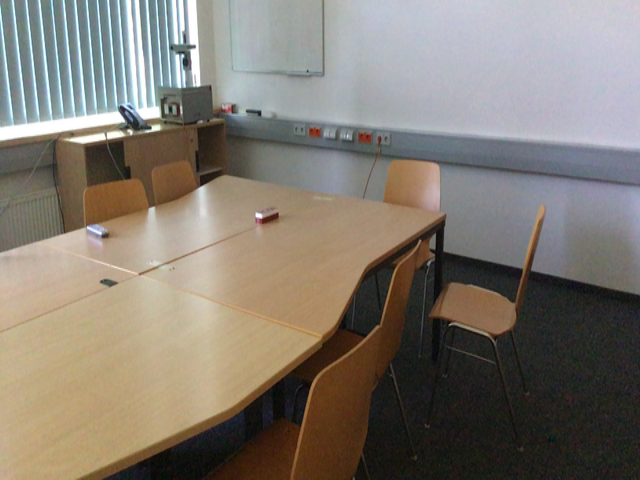
\includegraphics[width=.3\linewidth]{Figures/results/s1_a1/u0RAW_RGB.png}&
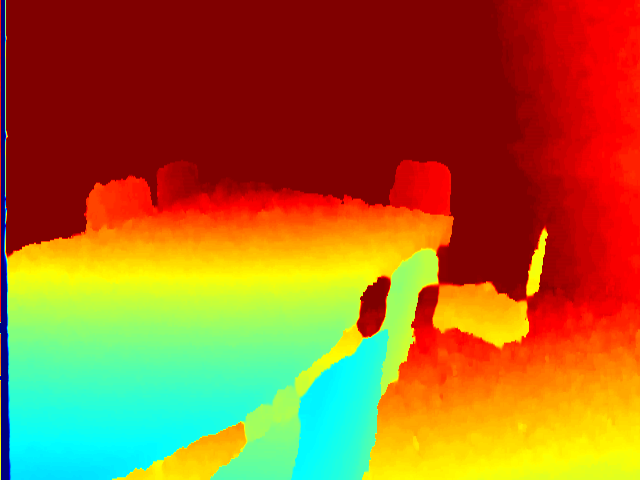
\includegraphics[width=.3\linewidth]{Figures/results/s1_a1/u0Truth.png}&
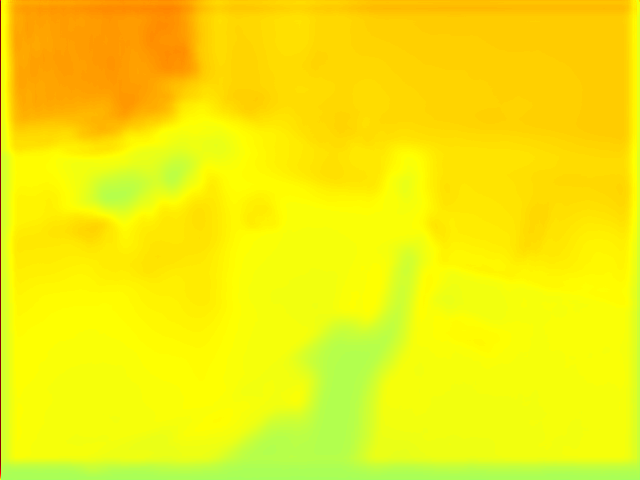
\includegraphics[width=.3\linewidth]{Figures/results/s1_a1/u0Predicted.png}\\[-1ex]
\rowname{E2 (b)}&
\includegraphics[width=.3\linewidth]{Figures/results/s1_a1/0RAW_RGB.png}&
\includegraphics[width=.3\linewidth]{Figures/results/s1_a1/0Truth.png}&
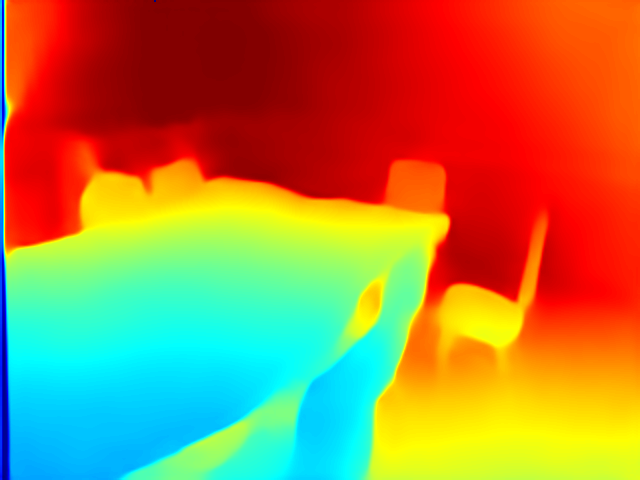
\includegraphics[width=.3\linewidth]{Figures/results/s1_a1/0Predicted.png}\\[-1ex]
\end{tabular}
\caption{\textbf{Influence of Structural Characteristics:} All the \textbf{E3} methods are in different  }%
\label{fig:results_E1_E2}
\end{figure}

\label{Chapter6:Influence_Structural_Char}
In this section we have investigated the Influence of Structural Characteristics of a pre-trained network backbone. \textbf{E1 - A1} model has no previously trained weights whereas \textbf{E2- A2} model has DenseNet backbone with pre trained weights only for the encoder part, which means, by evaluating \textbf{E1 - A1} against \textbf{E2 - A2} we can find out wheather the pre-trained backbone encoder model can have a influence over our results. One main significant different is in the decoder block, \textbf{A2} model is not trained on ImageNet as we discussed earlier in Section \ref{Chapter3:RelatedWork_NNModel} which implies the \textbf{A2} encoder has learnt Structural Characteristics feature from RBG images. Therefor we evaluate this influence of such pre-trained backbone. Therefore we train both the models with same SD\_v1 dataset with the train, validation and test set split of 80\%, 10\%  and 10\% respectively. Note that in \textbf{E2 - A2} case, we train only the decoder part. From the result in table \ref{table:Results_main} we see that the model performs gives a accuracy \textbf{a1} of only \textbf{0.22} which is 22 \% when compared with \textbf{A2} accuracy of \textbf{0.60}. Also the RMSE error is also high in \textbf{E1 - A1} compared to \textbf{E2 - A2}. Similarly the output from both the model in fig. \ref{fig:results_E3_E4} also shows  \textbf{E1 - A1} failed to perform. Important factor to notice is that, there were several layer parameters and hyper parameters where changed and tested before reaching the current \textbf{E1 - A2}. Due to the poor performance we did not document every step of model tuning of \textbf{E1 - A1} 

Observation: On a positive note for \textbf{E1 - A1} there are two things to be noted. First,  \textbf{E1 - A1} model can learn some structure characters as seen in the predicted image in fig. \ref{fig:results_E3_E4} \textbf{E1(a)} we notice that the chair could be identified to be closer than the wall behind. Second, we noticed that training and prediction is relatively  faster than \textbf{E2 - A2} model which means smaller network can give faster results. On the negative  side performance is very poor. 
Therefore, it is very clear that \textbf{E2 - A2} with DenseNet backbone outperforms \textbf{E1 - A1}. Since the accuracy of \textbf{E1 - A1} was extremely poor we believe that this is an effect of less data available for training, which gave us an motivation for SD\_v2  dataset to generate more data. Thus we believe for further experiments choosing \textbf{A2} model over \textbf{A1} would be beneficial. Which leads us to the second step of this study which is to answer, if we can train the network to reproduce the holes in the similar fashion to Structure Sensor. And we have a better working model \textbf{A2} but still not the best. Since as we see in Fig. \ref{fig:results_E1_E2} the sooth edges around the objects in the predicted frame. 
 


 

 \section{Effect of Camera Properties}
 \label{Chapter6:Transfer_Learning}
Second investigation was performed to find the influence of transfer learning. In this method we input depth image for the network was with holes, still keeping the primary objective in this second stage of experimental process of finding optimal model for the best results. In order to find the best working model, From the previous investigation we understood the impact of pre-trained backbone (encoder) in our case which is DenseNet, in this experiment we two different configuration changes only on decoder part by keeping the encoder unchanged. Initially in first experiment \textbf{E3 - A2\_Holes(N+S)}  we trained our decoder part with two datasets one from kinect sonsor (NYU\_v2) and Structure sensor (SD\_v2)and in the second experiment \textbf{E4 - A2\_Holes(S)} we only with Structure sensor (SD\_v2) dataset. By this we can study the effects and influence different camera properties in our results there by achieving optimal model for our task.

The results from the table \ref{table:Results_main} we notice that all the three accuracy of \textbf{E3 - A2\_Holes(N+S)} is higher than \textbf{E4 - A2\_Holes(S)} similarly both the error is also lower for \textbf{E3 - A2\_Holes(N+S)} which means \textbf{E3 - A2\_Holes(N+S)} perform better than  \textbf{E4 - A2\_Holes(S)}. But when we compare difference of these five metrics individually, we find that there are only small difference. For instance lets us consider RMSE, \textbf{E3 - A2\_Holes(N+S)} has error rate of \textbf{0.27} while \textbf{E4 - A2\_Holes(S)} error rate is \textbf{0.34} with difference \textbf{0.07}. In the same way for accuracy \textbf{a1}, the accuracy difference between both the configurations where only \textbf{0.06}, for \textbf{a2} is \textbf{0.03} and for \textbf{a3} is just \textbf{0.02}. 

But when we compare the resultant depth maps from these two experimental configurations, visually the difference are higher with respect to precision at the object boundaries which can be seen in the Fig.\ref{fig:results_E3_E4}  where \textbf{E3 (a) - E3(c)} represented the resultant output from \textbf{E3 - A2\_Holes(N+S)} and similarly  \textbf{E4 (a) - E4(c)} represented the output from \textbf{E4 - A2\_Holes(S)}. We notice two significant difference, first a blurred effect at object edges for the model trained only on SD\_v2 dataset, where as we get refined edges with \textbf{E4 - A2\_Holes(S)}. Secondly, we observe that our model \textbf{E3 - A2\_Holes(N+S)} has learnt the holes. What is more interesting is as we see in the Fig. \ref{fig:results_E3_E4} \textbf{E3 (b)} model can learn even the complex environment which is comprised of many pole looking structures (legs of chairs in a classroom environment).

Oservation: As we have seen that our \textbf{A2} model when trained with both dataset performs better than when trained on one dataset alone. On a positive note, we see that data from Kinect sensor has improved our results. On the other hand, when we consider the size of SD\_v2 compared with NVU\_v2, SD\_v2 is relatively small. So it is difficult to study and conclude the effect of camera properties. But what we can say is NYU\_v2 dataset has a significant impact in our result and our current model can be trained to higher precision even for regeneration of holes.



 
 \begin{figure} [h]
\settoheight{\tempdima}{\includegraphics[width=.32\linewidth]{example-image-a}}%
\centering\begin{tabular}{@{}c@{ }c@{ }c@{ }c@{}}
&\textbf{RGB} & \textbf{Truth} & \textbf{Predticted} \\
\rowname{E3 (a)}&
\includegraphics[width=.3\linewidth]{Figures/results/s2_Holes/0RAW_RGB.png}&
\includegraphics[width=.3\linewidth]{Figures/results/s2_Holes/0Truth.png}&
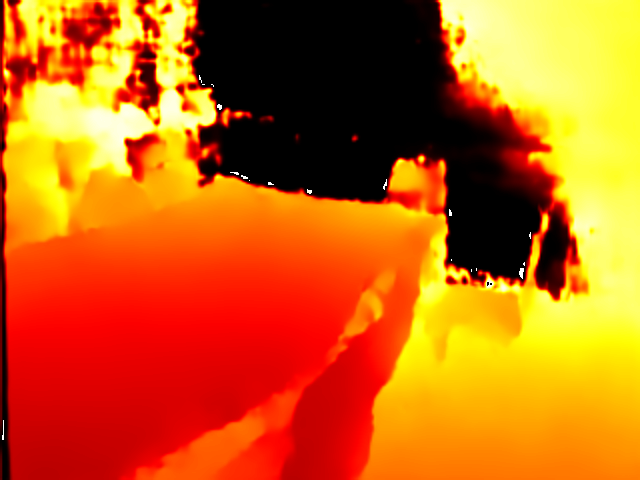
\includegraphics[width=.3\linewidth]{Figures/results/s2_Holes/0Predicted.png}\\[-1ex]
\rowname{E3 (b)}&
\includegraphics[width=.3\linewidth]{Figures/results/s2_Holes/1RAW_RGB.png}&
\includegraphics[width=.3\linewidth]{Figures/results/s2_Holes/1Truth.png}&
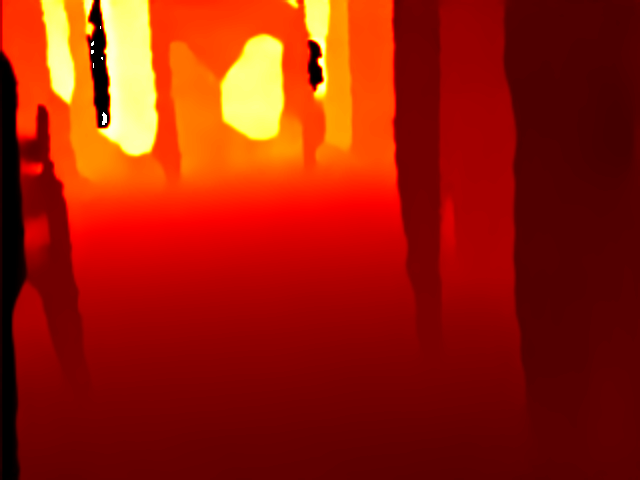
\includegraphics[width=.3\linewidth]{Figures/results/s2_Holes/1Predicted.png}\\[-1ex]
\rowname{E3 (c)}&
\includegraphics[width=.3\linewidth]{Figures/results/s2_Holes/2RAW_RGB.png}&
\includegraphics[width=.3\linewidth]{Figures/results/s2_Holes/2Truth.png}&
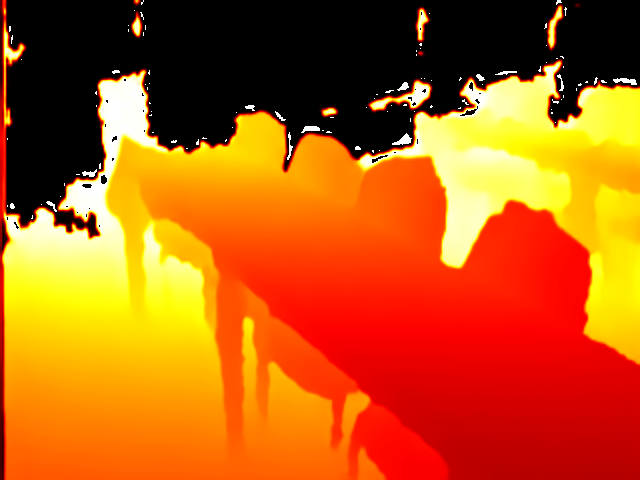
\includegraphics[width=.3\linewidth]{Figures/results/s2_Holes/2Predicted.png}\\[-1ex]
\rowname{E4 (a)}&
\includegraphics[width=.3\linewidth]{Figures/results/s3_noNyu/0RAW_RGB.png}&
\includegraphics[width=.3\linewidth]{Figures/results/s3_noNyu/0Truth.png}&
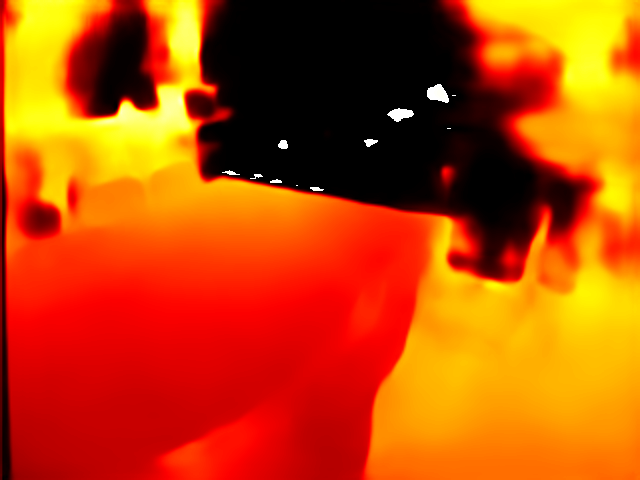
\includegraphics[width=.3\linewidth]{Figures/results/s3_noNyu/0Predicted.png}\\[-1ex]
\rowname{E4 (b)}&
\includegraphics[width=.3\linewidth]{Figures/results/s3_noNyu/1RAW_RGB.png}&
\includegraphics[width=.3\linewidth]{Figures/results/s3_noNyu/1Truth.png}&
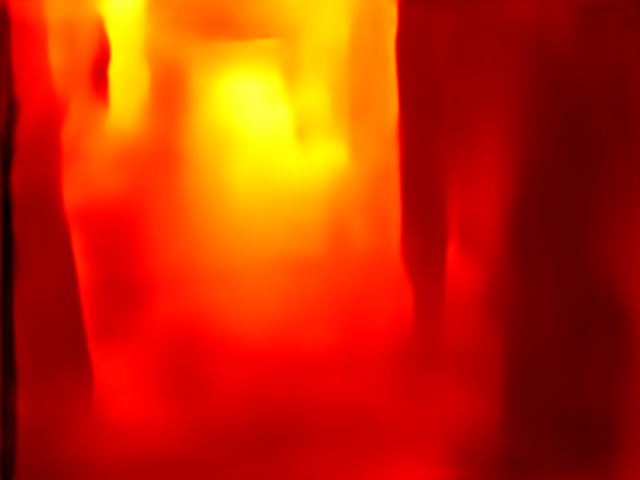
\includegraphics[width=.3\linewidth]{Figures/results/s3_noNyu/1Predicted.png}\\[-1ex]
\rowname{E4 (c)}&
\includegraphics[width=.3\linewidth]{Figures/results/s3_noNyu/2RAW_RGB.png}&
\includegraphics[width=.3\linewidth]{Figures/results/s3_noNyu/2Truth.png}&
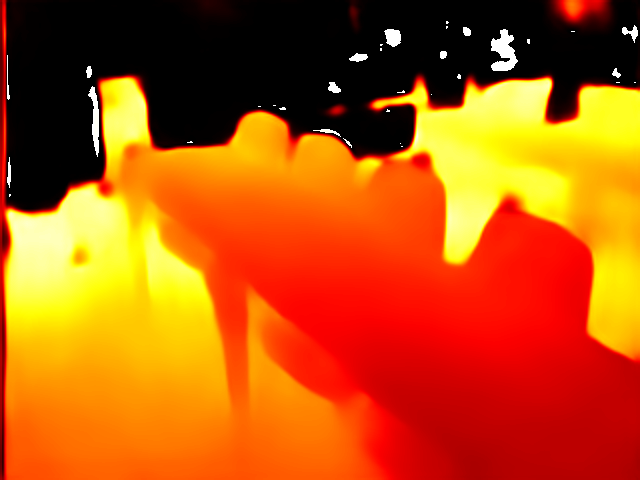
\includegraphics[width=.3\linewidth]{Figures/results/s3_noNyu/2Predicted.png}\\[-1ex]
\end{tabular}
\caption{\textbf{Investigation on hole regeneration method:} All the \textbf{E3} methods are in different  }%
\label{fig:results_E3_E4}
\end{figure}





\newpage
 \section{Hole Regeneration}
 \label{Chapter6:Hole_Regeneration}
Further more to improve the results for estimation of depth maps for 3D reconstruction, we study the importance/influence of effects of a probabilistic distribution (in other words neural network's output is a distribution of probable values ranging from 0.0 to 1.0 on a image level) over this regenerating holes. As described in section \ref{Chapter4:Dataset}, in order to have a holes recreated we mapped all the dead value or no pixel region as zero. Therefore we have two methods of pre-possessing carried out with two different input feature type, one with holes and another without holes. We tested the performance of \textbf{A2\_Holes} against the \textbf{A2\_NoHoles} models. In Fig. \ref{fig:results_S2} (a) - (c) we see that there a good reconstruction of the depth map were all the holes were interpolated to its neighboring pixel.  Fig. \ref{fig:results_S2} (d) - (f)  corresponds to the model with the holes as a input to the network. As we see in Fig \ref{fig:results_S2}, we compare \textbf{E5} and \textbf{E6}. We have used two different color maps for \textbf{E5} and \textbf{E6}. This is because in \textbf{E4} we wanted to highlight the difference between holes which were mapped to zero and the closest region in an image. 

From the table \ref{table:Results_main} we notice that the on an average the model \textbf{E3 (A2\_NoHoles)} performs better. When RMSE is taken into consideration we can clearly see that \textbf{E3 (A2\_NoHoles)} performs better with the RMSE of \textbf{0.10} which is \textbf{0.17} lower than the \textbf{E4 (A2\_Holes)} with RMSE of \textbf{0.27}. And when we notice our accuracy a1, a2 and a3 we see the similar results when compared. But when notice in the Fig. \ref{fig:results_S2} (d) - (f) we have visually good prediction. when investigated further why such hugh difference in the accuracy and error we found out the error lies in the object boundaries. As we see in the fig () there is a interpolation intermediate pixel from the zero value (holes which are mapped as zeros) till the actual depth. This effect is cause because of the probabilistic distribution method of neural network characteristic. We strongly this is one of there main factors contributing to the difference in the error and accuracy between \textbf{E5} and \textbf{E6}. Now that we understand why such effects can be seen for the generation of holes, it is very important us to answer if such approach is beneficial or not. Given such a problem of linear \notice{interpolating prediction} one possible solotion can be given by some post-filtering or post processing methods but the idea for the case of this study is to provide end to end approch as much as possible thereby exploiting the potential of the neural network. 

Therefore we see that given an input with holes the model can learn the holes from the given monocular input. But it results into \notice{interpolating prediction} which we believe makes the 3D reconstruction of a scene more difficult and demands further post processing techniques. This leads us to an conclusion that interpolating of pixel is a better approach than making the network learn to predict holes. In addition to this, one of the other motivation to try this approach was to eliminate the wall effect of depth maps  for the pixel farther than the distance limit, one approach for this solution could be taking a threshold just before the highest pixels. This solves the problem of having wall in out 3D reconstruction scene.

In summary, we believe that the comparing the two different input representation, \textbf{A2\_NoHoles} approach where the holes are interpolated with its neighboring pixels is beneficial.





\begin{figure} 
\settoheight{\tempdima}{\includegraphics[width=.32\linewidth]{example-image-a}}%
\centering\begin{tabular}{@{}c@{ }c@{ }c@{ }c@{}}
&\textbf{RGB} & \textbf{Truth} & \textbf{Predticted} \\
\rowname{E3 (a)}&
\includegraphics[width=.3\linewidth]{Figures/results/s2_NoHoles/0RAW_RGB.png}&
\includegraphics[width=.3\linewidth]{Figures/results/s2_NoHoles/0Truth.png}&
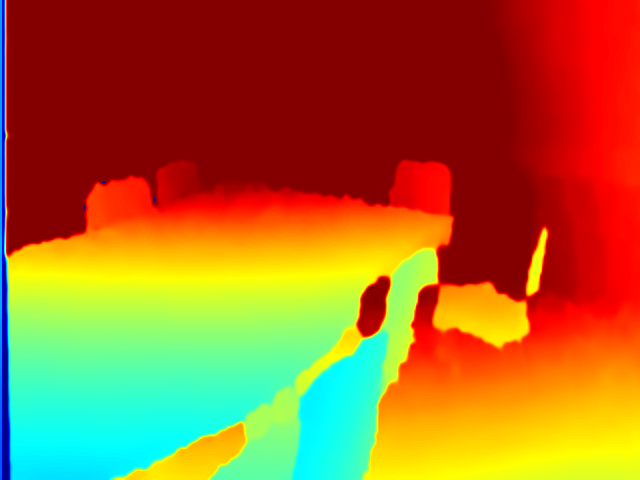
\includegraphics[width=.3\linewidth]{Figures/results/s2_NoHoles/0Predicted.png}\\[-1ex]
\rowname{E3 (b)}&
\includegraphics[width=.3\linewidth]{Figures/results/s2_NoHoles/1RAW_RGB.png}&
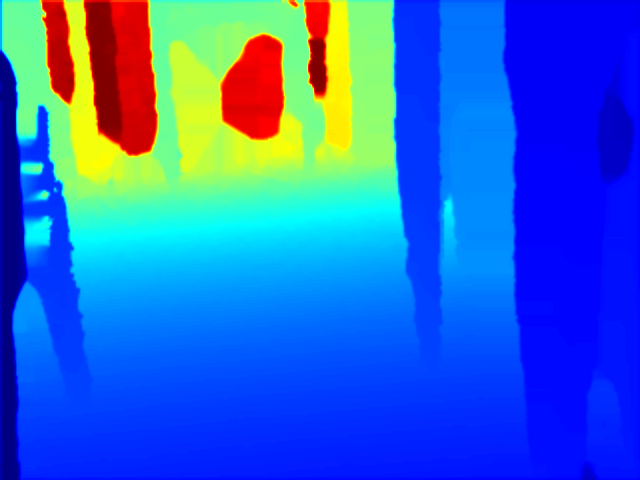
\includegraphics[width=.3\linewidth]{Figures/results/s2_NoHoles/1Truth.png}&
\includegraphics[width=.3\linewidth]{Figures/results/s2_NoHoles/1Predicted.png}\\[-1ex]
\rowname{E3 (c)}&
\includegraphics[width=.3\linewidth]{Figures/results/s2_NoHoles/2RAW_RGB.png}&
\includegraphics[width=.3\linewidth]{Figures/results/s2_NoHoles/2Truth.png}&
\includegraphics[width=.3\linewidth]{Figures/results/s2_NoHoles/2Predicted.png}\\[-1ex]
\rowname{E4 (d)}&
\includegraphics[width=.3\linewidth]{Figures/results/s2_Holes/0RAW_RGB.png}&
\includegraphics[width=.3\linewidth]{Figures/results/s2_Holes/0Truth.png}&
\includegraphics[width=.3\linewidth]{Figures/results/s2_Holes/0Predicted.png}\\[-1ex]
\rowname{E4 (e)}&
\includegraphics[width=.3\linewidth]{Figures/results/s2_Holes/1RAW_RGB.png}&
\includegraphics[width=.3\linewidth]{Figures/results/s2_Holes/1Truth.png}&
\includegraphics[width=.3\linewidth]{Figures/results/s2_Holes/1Predicted.png}\\[-1ex]
\rowname{E4 (f)}&
\includegraphics[width=.3\linewidth]{Figures/results/s2_Holes/2RAW_RGB.png}&
\includegraphics[width=.3\linewidth]{Figures/results/s2_Holes/2Truth.png}&
\includegraphics[width=.3\linewidth]{Figures/results/s2_Holes/2Predicted.png}\\[-1ex]
\end{tabular}
\caption{\textbf{Investigation on hole regeneration method:} All the \textbf{E3} methods are in different  }%
\label{fig:results_S2}
\end{figure}





%\section{Qualitative evaluation}

%Here we have evaluted our result with the state of the art in the table below 
% Chapter Template


\chapter{Conclusion}
\label{Chaptee7:Concluion}
The primary objective of this study is to achieve a best working model for a specific environment and task based system which in our case is depth estimation using IPad and Structure sensor for indoor scene. Through the process of various experimental study we have achieved a best working model for depth estimation using Neural Network which can work as good as Structure Sensor with an accuracy score of \textbf{0.98}. Along with the accuracy score, we also studied its performance by visual representation in 2D and 3D. The entire process of this study can be categorized in to three section.

First, we proposed a novel neural network architecture which is lower in complexity with respect to learning parameters. As an initial step we evaluated our proposed method against existing model architecture. Due to the lack of data for training, our proposed model did not work as good as state of the art approach. The result of this is discussed in Section \ref{Chapter6:Influence_Structural_Char}, which also gives an understanding, if the network with the pre-trained structural features can help in depth estimation. 

Second, we evaluated how well a model trained in Kinect sensor data can perform on Structure Sensor dataset thereby answering, if there a need for a task based model and dataset to be created or in other words, the influence of different environment specific models. We retrained the existing model which was pre trained with Kinect Sensor with Structure Sensor data and tested their performance with each other (one model trained only on SD another model trained both on NYU\_v2 and SD). The resuls shows that, there is a huge impact in terms of accuracy from the results discussed in Section \ref{Chapter6:Transfer_Learning} but when further tested against model only trained on NYU\_v2 dataset we see a significance impact of different camera properties which is discussed in Section \ref{Chapter6:ComapreS-F-A}. Thus from this, we conclude that a model must be tuned according to the given specific environment and task intended for the depth estimation case.

Thirdly, we proposed a novel idea to mimic the Structure Sensor by making the network learn the holes in the similar to sensor. Also keeping the focus of implementation of this depth estimation model for the task of 3D reconstruction in indoor environment we evaluated against standard approach of interpolating of holes to the nearest neighbour method. Model can learn and give a good prediction with high accuracy but with an artifact. We found that there is a intermediate pixel generated. The results are discussed in details in Section \ref{Chapter6:Hole_Regeneration}. This leads to a conclusion that we can only use such model with proper post processing or pre processing methods. Since for our study, it is always desired to have an end to end approach we believe the best solution approach would be to have label input for depth maps with no holes. 

Thus experimenting on different testing conditions we conclude that, having a pre-trained backbone even when designed for different task and environment has significant improvement in learning structural dependency in depth estimation tasks but not the depth feature. This is because, there is a significance influence of different camera properties hence environment specific dataset must be needed for better performance. Finally for 3D reconstruction, approach with no holes has proves to be beneficial to provide a end to end solution.

 
% Chapter Template


\chapter{Image Gallery}

\label{Chapter8:Image_Gallery} 

%----------------------------------------------------------------------------------------
%	THESIS CONTENT - APPENDICES
%----------------------------------------------------------------------------------------

\appendix % Cue to tell LaTeX that the following "chapters" are Appendices

% Include the appendices of the thesis as separate files from the Appendices folder
% Uncomment the lines as you write the Appendices

%\bibliography{reference}
%% Appendix A

\chapter{Frequently Asked Questions} % Main appendix title

\label{AppendixA} % For referencing this appendix elsewhere, use \ref{AppendixA}

\section{How do I change the colors of links?}

The color of links can be changed to your liking using:

{\small\verb!\hypersetup{urlcolor=red}!}, or

{\small\verb!\hypersetup{citecolor=green}!}, or

{\small\verb!\hypersetup{allcolor=blue}!}.

\noindent If you want to completely hide the links, you can use:

{\small\verb!\hypersetup{allcolors=.}!}, or even better: 

{\small\verb!\hypersetup{hidelinks}!}.

\noindent If you want to have obvious links in the PDF but not the printed text, use:

{\small\verb!\hypersetup{colorlinks=false}!}.

%\include{Appendices/AppendixB}
%\include{Appendices/AppendixC}

%----------------------------------------------------------------------------------------
%	BIBLIOGRAPHY
%----------------------------------------------------------------------------------------
%\bibliographystyle{ieeetr}
\printbibliography[heading=bibintoc]

%----------------------------------------------------------------------------------------

\end{document}  
